\chapter{Definite Integrals}

\section{Concept of Definite Integrals and their Relationship with Indefinite Integrals}

\subsection*{Concept of Definite Integrals}

A lot of practical problems, for example finding area and volumes, can be
reduced to finding the limit of a certain type of sum. Let's take finding area
as an example to explain the method of solving this kind of problem, and hence
introduce the concept of definite integrals.

\begin{center}
    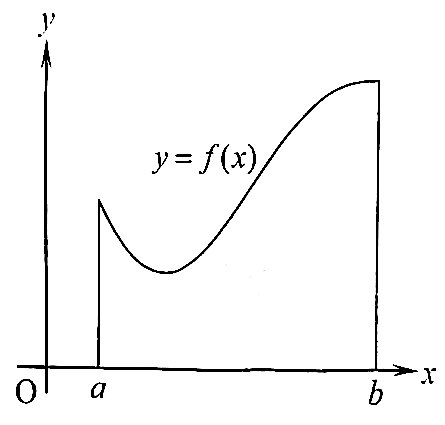
\includegraphics[scale=0.3]{assets/28-3.jpg}
\end{center}

Shown in the diagram above (shaded area) is the area bounded by the line $x =
    a$, $x = b$, $y = 0$, and the curve $y = f(x)$ where $f(x) \geq 0$. This kind
of graph is called the curved trapezoid.

\begin{center}
    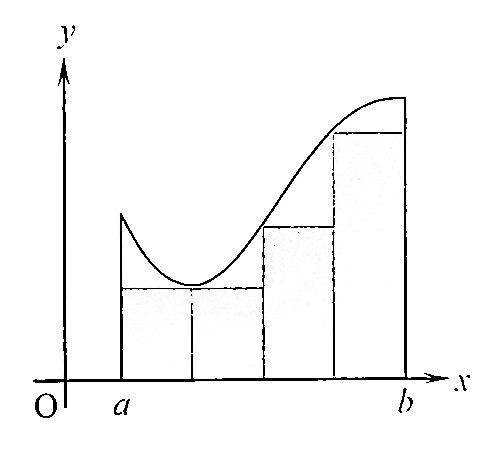
\includegraphics[scale=0.3]{assets/28-1.jpg}
    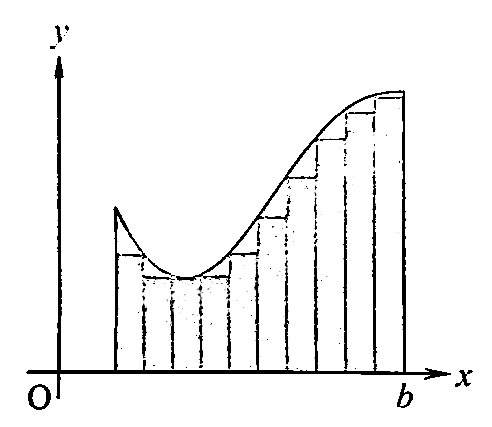
\includegraphics[scale=0.3]{assets/28-2.jpg}
    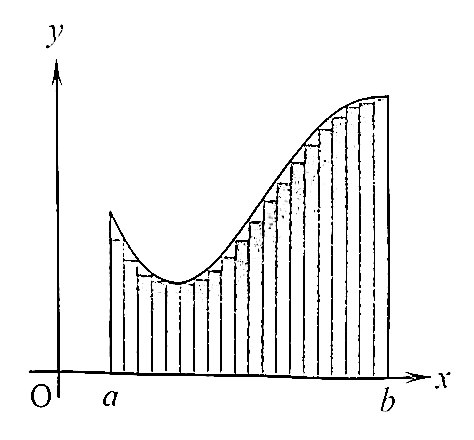
\includegraphics[scale=0.3]{assets/28-4.jpg}
\end{center}

As shown in the diagram above, in order to find the area of this curved
trapezoid, we can split it into multiple small curved trapezoid, each of them
being substituted by their respective rectangular shape. As such, an
approximate value of the area of the curved trapezoid can be acquired by
summing up of the area of each rectangle. As the curved trapezoid is being
split into smaller and smaller pieces, the approximate value we get will get
closer and closer to its actual area.

With this concept in mind, we can split the interval $[a, b]$ into $n$ smaller
interval $[x_0, x_1]$, $[x_1, x_2]$, $\cdots$, $[x_{n-1}, x_n]$ where $x_0 =
    a$, $x_n = b$. From drawing lines that are perpendicular to the $x$-axis
through the points $x_1$, $x_2$, $\cdots$, $x_{n-1}$, we can split the curved
trapezoid into $n$ smaller curved trapezoid.

\begin{center}
    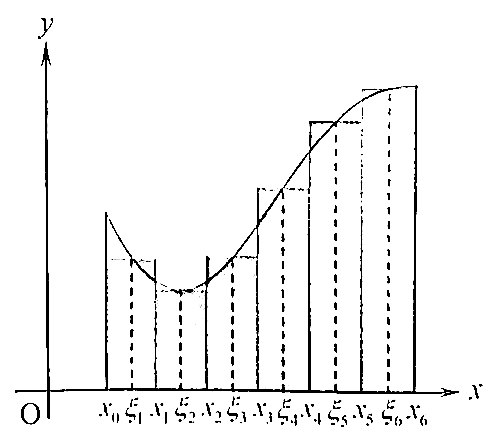
\includegraphics[scale=0.3]{assets/28-5.jpg}
\end{center}

Choose any point $\xi_i$ in the $i$-th interval $[x_{i-1}, x_i]$, then the area
$\Delta A$ of the $i$-th curved trapezoid can be approximated by the area of
the rectangle with width $\Delta x_i = x_i - x_{i-1}$ and height $f(\xi_i)$, as
shown in the diagram above, i.e.
\begin{cequation}
    \Delta A_i \approx f(\xi_i)\Delta x
\end{cequation}
And the approximated value of the area of the original curved trapezoid is the sum of the area of all the smaller rectangle, i.e.
\begin{cequation}
    A = \sum_{i=1}^n \Delta A_i \approx \sum_{i=1}^n f(\xi_i)\Delta x
\end{cequation}

As the number of smaller interval $n$ increases and the width of each interval
decreases, the approximated value of the area of the original curved trapezoid
gets closer and closer to its actual area. To find the value of $A$, we split
the interval $[a, b]$ into indefinitely many smaller interval such that $\Delta
    x \to 0$ (i.e. $n \to \infty$), hence the area of the original curved trapezoid
can be defined as the limit of the sum of the area of all the smaller
rectangle, i.e.
\begin{cequation}
    A = \lim_{n \to \infty} \sum_{i=1}^n f(\xi_i)\Delta x
\end{cequation}

This limit is called the definite integral of $f(x)$ from $a$ to $b$, and is
denoted by the symbol $\displaystyle\int_a^b f(x) dx$, i.e.
\begin{cequation}
    \int_a^b f(x) dx = \lim_{n \to \infty} \sum_{i=1}^n f(\xi_i)\Delta x
\end{cequation}
where $f(x)$ is called the integrand, $[a, b]$ is called the interval of integration, $a$ and $b$ are called the lower and upper limits of integration respectively.

If $f(x) \geq 0$ in the interval $[a, b]$, we know from the above discussion
that the value of the definite integral $\displaystyle\int_a^b f(x) dx$ is the
area of the curved trapezoid bounded by the curve $y = f(x)$, the $x$-axis, and
the lines $x = a$ and $x = b$, i.e. $A = \displaystyle\int_a^b f(x) dx$.

\vspace{0.5cm}
\begin{vwcol}[widths={0.7,0.3},justify=flush,rule=0pt,indent=1em]
    If $f(x) \leq 0$ in the interval $[a, b]$, as shown in the diagram on the right-hand-side,
    $f(\xi_i)\Delta x$ is the negative value of the area of the $i$-th smaller
    rectangle. Hence, the definite integral $\displaystyle\int_a^b f(x) dx$ is
    negative, and its absolute value is the area of the curved trapezoid bounded by
    the curve $y = f(x)$, the $x$-axis, and the lines $x = a$ and $x = b$, i.e. $A
        = -\displaystyle\int_a^b f(x) dx$.

    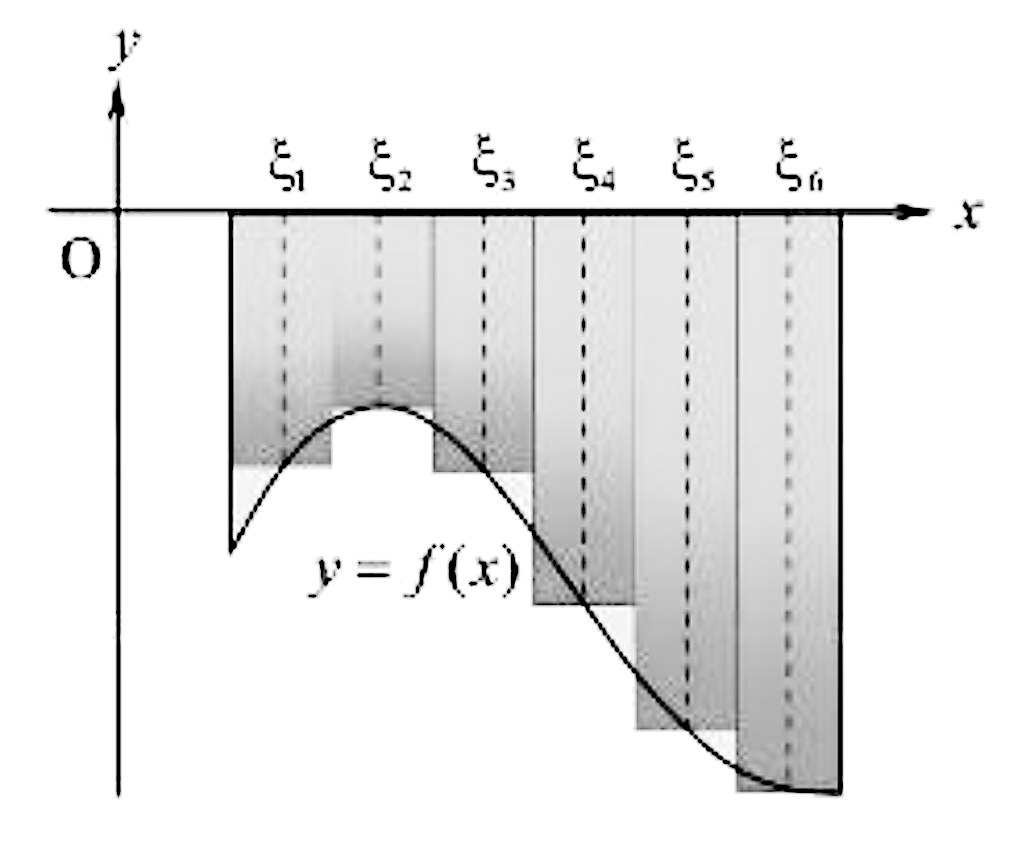
\includegraphics[scale=0.15]{assets/28-4.png}
\end{vwcol}

\newpage

\subsection*{The Relationship between Definite Integrals and Indefinite Integrals}

The definite integrals and the indefinite integrals has inseparable
relationship between them. Consider the case of finding the area of curved
trapezoid. Let $x_0 > a$ and $f(x) \geq 0$. The area of the curved trapezoid
bounded by the curve $y = f(x)$, the $x$-axis, and the lines $x = a$, $x = x_0$
and $y = 0$ is $A(x_0) = \displaystyle\int_a^{x_0} f(x) dx$.

\vspace{0.5cm}
\begin{vwcol}[widths={0.6,0.4},justify=flush,rule=0pt,indent=1em]
    When $x_0$ changes, the area $A(x_0)$ also changes. From the diagram above, we
    know that
    \begin{cequation}
        m\Delta x \leq A(x_0 + \Delta x) - A(x_0) \leq M\Delta x,
    \end{cequation}
    where $m$ and $M$ are the minimum and maximum values of $f(x)$ in the interval $[x_0, x_0 + \Delta x]$. Hence,
    \begin{cequation}
        m \leq \dfrac{A(x_0 + \Delta x) - A(x_0)}{\Delta x} \leq M.
    \end{cequation}

    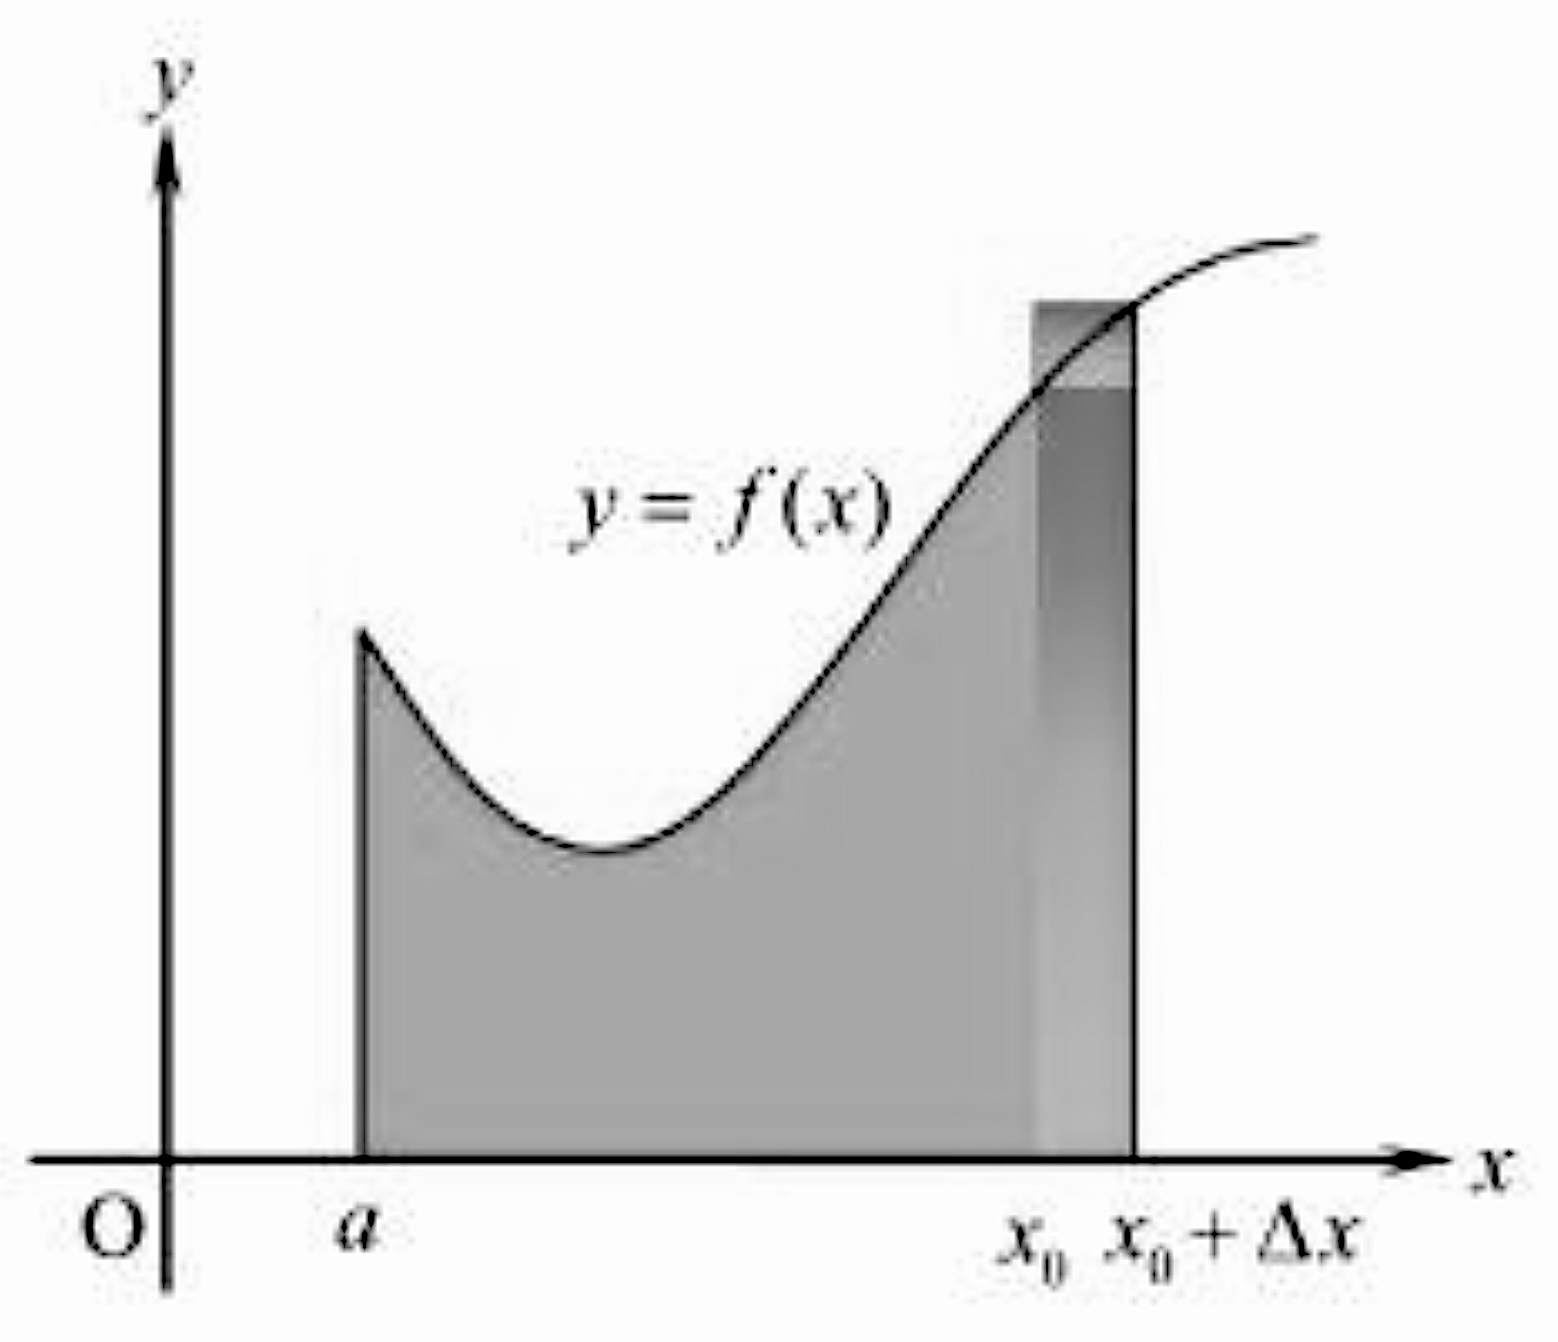
\includegraphics[scale=0.1]{assets/28-7.png}
\end{vwcol}
\vspace{0.5cm}

Apparently, as $\Delta x$ approaches 0, both $m$ and $M$ approach $f(x_0)$.
Besides, from the definition of derivative, \\$\lim_{\Delta x \to 0}
\dfrac{A(x_0 + \Delta x) - A(x_0)}{\Delta x} = A'(x_0)$. Hence, we get $A'(x_0)
= f(x_0)$. This relational expression is true for any $x_0 > a$. In other
    words, $A'(x) = f(x)$, i.e. the derivative of the area function $A(x)$ is the
    integrand $f(x)$.

    Let $\displaystyle\int f(x)d x = F(x) + C$, i.e. $F(x)$ is the primitive of
$f(x)$. Then, from $A'(x) = f(x) = F'(x)$, we get $A(x) = F(x) + C$, where $C$
    is a constant. When $A(a) = 0$, $x = a$, we get $C = -F(a)$. Hence, $C =
-F(a)$, i.e. for any $x_0 > a$, we get $A(x_0) = F(x_0) - F(a)$.

    Let $x_0 = b$, we get $A(b) = \displaystyle\int_a^b f(x) dx = F(b) - F(a)$.
    This relational expression is true for any continuous function $f(x)$. In order
    to make the relational expression true for any $a$ and $b$, when $a > b$, the
    following definition is made.
    \begin{center}
        \framebox{

            \parbox[t][1.3cm]{6cm}{ \addvspace{0.2cm} \centering $\displaystyle\int_a^b f(x) dx
                    = -\int_b^a f(x) dx$ }}
    \end{center}

    Above all are the relationship between definite integrals and indefinite
    integrals, i.e. \vspace{-0.9em}
    \begin{center}
        \framebox{

            \parbox[t][1.3cm]{9cm}{ \addvspace{0.2cm} \centering If $\displaystyle\int f(x) dx
                    = F(x) + C$, then $\displaystyle\int_a^b f(x) dx = F(b) - F(a)$. }}
    \end{center}
    This relationship is called the fundamental theorem of calculus. Generally, we
    express the expression as follows:
    \begin{cequation}
        \int_a^b f(x) dx = \big[F(x)\big]_a^b = F(b) - F(a).
    \end{cequation}
    where $F(x)$ is any primitive of $f(x)$.

    When finding the definite integral $\displaystyle\int_a^b f(x) dx$, we only
    have to find any primitive $F(x)$ of $f(x)$. The other primitive of $f(x)$ can
    be expressed as $F(x) + C$, where $C$ is a constant. Hence, the definite
    integral $\displaystyle\int_a^b f(x) dx$ is independent of the choice of
    primitive of $f(x)$. But,
    \begin{flalign*}
         & \big[F(x) + C\big]_a^b = [F(b) + C] - [F(a) + C] = F(b) - F(a)
    \end{flalign*}
    Hence, the value of the definite integral has nothing to do with the constant $C$. The value of the definite integral remains the same no matter which primitive of $f(x)$ is chosen.

    Note that $\big[F(x)\big]_a^b$ can also be written as $F(x)\big|_a^b$.

    \newpage
    \subsection{Practice 2}

\begin{enumerate}
    \begin{multicols}{2}
        \item $\displaystyle\int_2^8 x d x$
        \sol{}
        \begin{flalign*}
            I & = \left[\dfrac{1}{2}x^2\right]_2^8 & \\
              & = \dfrac{1}{2}(64 - 4)             & \\
              & = 30
        \end{flalign*}

        \item $\displaystyle\int_{-2}^4 x^3 d x$
        \sol{}
        \begin{flalign*}
            I & = \left[\dfrac{1}{4}x^4\right]_{-2}^4 & \\
              & = \dfrac{1}{4}(256 - 16)              & \\
              & = 60
        \end{flalign*}
    \end{multicols}
    \begin{multicols}{2}
        \item $\displaystyle\int_{-\pi}^\pi \cos x d x$
        \sol{}
        \begin{flalign*}
            I & = \bigg[\sin x\bigg]_{-\pi}^\pi & \\
              & = \sin\pi - \sin(-\pi)          & \\
              & = 0 - 0                         & \\
              & = 0
        \end{flalign*}

        \item $\displaystyle\int_0^{\frac{\pi}{4}} \sec ^2 x d x$
        \sol{}
        \begin{flalign*}
            I & = \bigg[\tan x\bigg]_0^{\frac{\pi}{4}} & \\
              & = \tan\dfrac{\pi}{4} - \tan 0          & \\
              & = 1 - 0                                & \\
              & = 1
        \end{flalign*}
    \end{multicols}
\end{enumerate}
    \subsection{Exercise 28.1}

\begin{enumerate}
    \begin{multicols}{2}
        \item $\displaystyle\int_{-2}^4 x^2 d x$
        \sol{}
        \begin{flalign*}
            I & = \left[\dfrac{1}{3}x^3\right]_{-2}^4 & \\
              & = \dfrac{1}{3}(64 + 8)                & \\
              & = 24
        \end{flalign*}
        \item $\displaystyle\int_1^4 \dfrac{1}{x^2} d x$
        \sol{}
        \begin{flalign*}
            I & = \left[-\dfrac{1}{x}\right]_1^4 & \\
              & = -\dfrac{1}{4} + 1              & \\
              & = \dfrac{3}{4}
        \end{flalign*}
    \end{multicols}

    \begin{multicols}{2}
        \item $\displaystyle\int_4^9 \sqrt{x} d x$
        \sol{}
        \begin{flalign*}
            I & = \left[\dfrac{2}{3}x^{\frac{3}{2}}\right]_4^9 & \\
              & = \dfrac{2}{3}(27 - 8)                         & \\
              & = \dfrac{38}{3}
        \end{flalign*}

        \item $\displaystyle\int_1^{27} \dfrac{1}{\sqrt[3]{x^5}} d x$
        \sol{}
        \begin{flalign*}
            I & = \left[-\dfrac{3}{2}x^{-\frac{2}{3}}\right]_1^{27} & \\
              & = -\dfrac{3}{2}\left(\dfrac{1}{9} - 1\right)        & \\
              & = \dfrac{4}{3}
        \end{flalign*}
    \end{multicols}
    \newpage
    \begin{multicols}{2}
        \item $\displaystyle\int_0^{\frac{\pi}{3}} \cos x d x$
        \sol{}
        \begin{flalign*}
            I & = \bigg[\sin x\bigg]_0^{\frac{\pi}{3}} & \\
              & = \sin\dfrac{\pi}{3} - \sin 0          & \\
              & = \dfrac{\sqrt{3}}{2} - 0              & \\
              & = \dfrac{\sqrt{3}}{2}
        \end{flalign*}

        \item $\displaystyle\int_{-\frac{\pi}{4}}^{\frac{\pi}{2}} \sin x d x$
        \sol{}
        \begin{flalign*}
            I & = \bigg[-\cos x\bigg]_{-\frac{\pi}{4}}^{\frac{\pi}{2}} & \\
              & = -\cos\dfrac{\pi}{2} - (-\cos(-\frac{\pi}{4}))        & \\
              & = 0 + \dfrac{\sqrt{2}}{2}                              & \\
              & = \dfrac{\sqrt{2}}{2}
        \end{flalign*}
    \end{multicols}

    \begin{multicols}{2}
        \item $\displaystyle\int_0^2 e^x d x$
        \sol{}
        \begin{flalign*}
            I & = e^2 - e^0 & \\
              & = e^2 - 1
        \end{flalign*}
        \vfill{}\null{}
        \columnbreak{}
        \item $\displaystyle\int_{\frac{\pi}{4}}^{\frac{\pi}{2}} \operatorname{cosec}^2 x d x$
        \sol{}
        \begin{flalign*}
            I & = \bigg[-\cot x\bigg]_{\frac{\pi}{4}}^{\frac{\pi}{2}} & \\
              & = -\cot\frac{\pi}{2} + \cot\frac{\pi}{4}              & \\
              & = 0 + 1                                               & \\
              & = 1
        \end{flalign*}
    \end{multicols}

    \begin{multicols}{2}
        \item $\displaystyle\int_1^2 \dfrac{1}{x} d x$
        \sol{}
        \begin{flalign*}
            I & = = \bigg[\ln|x|\bigg]_1^2 & \\
              & = \ln 2 - \ln 1            & \\
              & = \ln 2
        \end{flalign*}

        \item $\displaystyle\int_0^2 \dfrac{1}{x+1} d x$
        \sol{}
        \begin{flalign*}
            I & = \bigg[\ln|x+1|\bigg]_0^2 & \\
              & = \ln 3 - \ln 1            & \\
              & = \ln 3                    & \\
        \end{flalign*}
    \end{multicols}
\end{enumerate}

\newpage


    \section{Properties and Calculations of Definite Integrals}

    \subsection*{Properties of Definite Integrals}

    \noindent \hspace{1.2em}\textit{The definite integrals have the following basic properties:}

    \begin{center}
        \framebox{

            \parbox[t][1.3cm]{10cm}{ \addvspace{0.2cm}\hspace{10pt}\textbf{Property 1}
                \hspace{10pt} $\displaystyle\int_a^b kf(x) dx = k\int_a^b f(x) dx$}}
    \end{center}
    \begin{center}
        \framebox{

        \parbox[t][1.3cm]{10cm}{ \addvspace{0.2cm}\hspace{10pt} \textbf{Property 2}
        \hspace{10pt} $\displaystyle\int_a^b [f(x) \pm g(x)] dx = \int_a^b f(x) dx \pm
            \int_a^b g(x) dx$}}
    \end{center}
    \begin{center}
        \framebox{

            \parbox[t][1.3cm]{10cm}{ \addvspace{0.25cm}\hspace{10pt}\textbf{Property 3}
                \hspace{10pt} $\displaystyle\int_c^a f(x) dx + \int_b^c f(x) dx = \int_b^a f(x)
                    dx$}}
    \end{center}

    \subsection{Practice 3}

\noindent \hspace{1.2em}\textit{
    Find the extreme values of the following functions (Question 1 to 4):
}

\begin{enumerate}
    \item $f(x)=x^2+x-6$
    \item $f(x)=2-x-x^2$
    \item $f(x)=\dfrac{1}{3} x^3-\dfrac{1}{2} x^2-2x+2$
    \item $f(x)=4 x-3 x^3$
\end{enumerate}

\noindent \hspace{1.2em}\textit{Find the coordinates of the extreme points of the following functions (Question 5 to 6):}
\begin{enumerate}[resume]
    \item $y=2 x^3-3 x^2-12 x-7$
    \item $y=x+\dfrac{1}{x}$
\end{enumerate}



    \subsection*{Integration by Substitution}

    In the last chapter, we have learned how to solve indefinite integrals using
    the method of integration by substitution: $\displaystyle\int f(g(x))g'(x)dx =
\int f(u)du$ where $u = g(x)$. From the basic theorem of calculus, the method
    of integration by substitution of definite integrals can be derived:
    \begin{center}
        \framebox{

            \parbox[t][1.3cm]{9cm}{ \addvspace{0.2cm} \centering $\displaystyle\int_a^b
                    f(g(x))g'(x)dx = \int_{g(a)}^{g(b)} f(u)du$ }}
    \end{center}
    \vspace{0.9em}
    The method of integration by substitution of definite integrals is similar to
    that of indefinite integrals. The only difference is that the limits of
    integration are changed accordingly.

    \subsection{Practice 4}

\noindent \hspace{1.2em}\textit{Find the absolute maximum value and the absolute minimum value of the following functions (Question 1 to 2):}
\begin{enumerate}
    \item $f(x) = 3x^3 - 9x + 5$, $[-2, 2]$
    \item $f(x) = x^4 - 2x^2 + 5$, $[-2, 3]$
    \item If $x + y = 8$, find the absolute minimum value of $x^2 + y^2$.
    \item A metal wire with a length of $100$cm is bent into a rectangle. Find the width
          and the length of the rectangle so that the area of the rectangle is the
          largest.
\end{enumerate}

    \newpage

    \subsection{Exercise 28.2}

\begin{enumerate}
    \begin{multicols}{2}
        \item $\displaystyle\int_0^4\left(x^2-2 x\right) d x$
        \sol{}
        \begin{flalign*}
            I & = \bigg[\dfrac{1}{3}x^3 - x^2\bigg]_0^4 & \\
              & = \dfrac{64}{3} - 16                    & \\
              & = \dfrac{16}{3}
        \end{flalign*}
        \item $\displaystyle\int_1^4 \dfrac{2 x^2-3 \sqrt{x}+1}{x} d x$
        \sol{}
        \begin{flalign*}
            I & = \int_1^4 \left(2x - 3x^{-\frac{1}{2}} + x^{-1}\right) d x & \\
              & = \bigg[x^2 - 6\sqrt{x} + \ln|x|\bigg]_1^4                  & \\
              & = 16 - 12 + \ln 4 - 1 + 6 - \ln 1                           & \\
              & = 9 + \ln 4
        \end{flalign*}
    \end{multicols}

    \begin{multicols}{2}
        \item $\displaystyle\int_{-3}^3(x+3)^2 d x$
        \sol{}

        Let $u = x + 3$, $du = dx$.

        When $x = -3$, $u = 0$.

        When $x = 3$, $u = 6$.
        \begin{flalign*}
            I & = \int_0^6 u^2 d u                & \\
              & = \bigg[\dfrac{1}{3}u^3\bigg]_0^6 & \\
              & = 72
        \end{flalign*}

        \item $\displaystyle\int_{-1}^1(2+x)\left(2-x^2\right) d x$
        \sol{}
        \begin{flalign*}
            I & = \int_{-1}^1\left(4 - 2x^2 + 2x - x^3\right)dx                             & \\
              & = \bigg[4x - \dfrac{2}{3}x^3 + x^2 - \dfrac{1}{4}x^4\bigg]_{-1}^1           & \\
              & = 4 - \dfrac{2}{3} + 1 - \dfrac{1}{4} + 4 - \dfrac{2}{3} - 1 + \dfrac{1}{4} & \\
              & = \dfrac{20}{3}
        \end{flalign*}
    \end{multicols}

    \begin{multicols}{2}
        \item $\displaystyle\int_0^{\frac{\pi}{2}}(2 \sin 3 \theta-3 \cos 2 \theta) d \theta$
        \sol{}
        \begin{flalign*}
            I & = \bigg[-\dfrac{2}{3}\cos 3\theta - \dfrac{3}{2}\sin 2\theta\bigg]_0^{\frac{\pi}{2}} & \\
              & = \dfrac{2}{3} + \dfrac{3}{2} + \dfrac{2}{3}                                         & \\
              & = \dfrac{13}{6}
        \end{flalign*}
        \vfill{}\null{}
        \columnbreak{}

        \item $\displaystyle\int_0^{\frac{\pi}{3}} \tan \theta d \theta$
        \sol{}
        \begin{flalign*}
            I & = \int_0^{\frac{\pi}{3}} \dfrac{\sin \theta}{\cos \theta} d \theta &
        \end{flalign*}
        Let $u = \cos \theta$, $du = -\sin \theta d \theta$.

        When $\theta = 0$, $u = 1$.

        When $\theta = \dfrac{\pi}{3}$, $u = \dfrac{1}{2}$.
        \begin{flalign*}
            I & = -\int_1^{\frac{1}{2}} \dfrac{1}{u} d u & \\
              & = -\bigg[\ln|u|\bigg]_1^{\frac{1}{2}}    & \\
              & = -\ln\dfrac{1}{2} + \ln 1               & \\
              & = \ln 2
        \end{flalign*}
    \end{multicols}

    \newpage

    \begin{multicols}{2}
        \item $\displaystyle\int_0^1\left(e^x-1\right)^2 d x$
        \sol{}
        \begin{flalign*}
            I & = \int_0^1\left(e^{2x} - 2e^x + 1\right) d x    & \\
              & = \bigg[\dfrac{1}{2}e^{2x} - 2e^x + x\bigg]_0^1 & \\
              & = \dfrac{1}{2}e^2 - 2e + 1 - \dfrac{1}{2} + 2   & \\
              & = \dfrac{1}{2}e^2 - 2e + \dfrac{5}{2}           & \\
              & = \dfrac{e^2 - 4e + 5}{2}
        \end{flalign*}
        \vfill{}\null{}

        \item $\displaystyle\int_1^4 \dfrac{2}{4 x-1} d x$
        \sol{}

        Let $u = 4x - 1$, $du = 4dx$.

        When $x = 1$, $u = 3$.

        When $x = 4$, $u = 15$.
        \begin{flalign*}
            I & = \dfrac{1}{2}\int_3^{15} \dfrac{1}{u} d u & \\
              & = \dfrac{1}{2}\bigg[\ln|u|\bigg]_3^{15}    & \\
              & = \dfrac{1}{2}(\ln 15 - \ln 3)             & \\
              & = \dfrac{1}{2}\ln 5
        \end{flalign*}
    \end{multicols}

    \begin{multicols}{2}
        \item $\displaystyle\int_{-1}^3 \sqrt{2 x+3} d x$
        \sol{}

        Let $u = 2x + 3$, $du = 2dx$.

        When $x = -1$, $u = 1$.

        When $x = 3$, $u = 9$.
        \begin{flalign*}
            I & = \dfrac{1}{2}\int_1^9 \sqrt{u} d u           & \\
              & = \dfrac{1}{3}\bigg[u^{\frac{3}{2}}\bigg]_1^9 & \\
              & = \dfrac{1}{3}(27 - 1)                        & \\
              & = \dfrac{26}{3}
        \end{flalign*}

        \item $\displaystyle\int_1^2 \dfrac{1}{(2 x-1)^3} d x$
        \sol{}

        Let $u = 2x - 1$, $du = 2dx$.

        When $x = 1$, $u = 1$.

        When $x = 2$, $u = 3$.
        \begin{flalign*}
            I & = \dfrac{1}{2}\int_1^3 u^{-3} d u                & \\
              & = -\dfrac{1}{4}\bigg[u^{-2}\bigg]_1^3            & \\
              & = -\dfrac{1}{4}\left(\dfrac{1}{9} - 1\right)     & \\
              & = -\dfrac{1}{4} \cdot \left(-\dfrac{8}{9}\right) & \\
              & = \dfrac{2}{9}
        \end{flalign*}
    \end{multicols}

    \begin{multicols}{2}
        \item $\displaystyle\int_{-1}^1 x^2\left(x^3-1\right)^4 d x$
        \sol{}

        Let $u = x^3 - 1$, $du = 3x^2dx$.

        When $x = -1$, $u = -2$.

        When $x = 1$, $u = 0$.
        \begin{flalign*}
            I & = \dfrac{1}{3}\int_{-2}^0 u^4 d u     & \\
              & = \dfrac{1}{15}\bigg[u^5\bigg]_{-2}^0 & \\
              & = \dfrac{32}{15}
        \end{flalign*}
        \columnbreak{}

        \item $\displaystyle\int_1^6 x \sqrt{3 x-2} d x$
        \sol{}

        Let $u = 3x - 2$, $du = 3dx$, $x = \dfrac{u + 2}{3}$.

        When $x = 1$, $u = 1$.

        When $x = 6$, $u = 16$.
        \begin{flalign*}
            I & = \dfrac{1}{3}\int_1^{16} \dfrac{u + 2}{3}\sqrt{u} d u                                     & \\
              & = \dfrac{1}{9}\int_1^{16} \left(u^{\frac{3}{2}} + 2u^{\frac{1}{2}}\right) d u              & \\
              & = \dfrac{1}{9}\bigg[\dfrac{2}{5}u^{\frac{5}{2}} + \dfrac{4}{3}u^{\frac{3}{2}}\bigg]_1^{16} & \\
              & = \dfrac{1}{9}\left(\dfrac{2048}{5} + \dfrac{256}{3} - \dfrac{2}{5} - \dfrac{4}{3}\right)  & \\
              & = \dfrac{274}{5}
        \end{flalign*}
    \end{multicols}

    \newpage
    \item $\displaystyle\int_{-\frac{\pi}{4}}^{\frac{\pi}{4}} \sin ^2 \theta d \theta$
          \sol{}
          \begin{flalign*}
              I & = \dfrac{1}{2}\int_{-\frac{\pi}{4}}^{\frac{\pi}{4}} (1 - \cos 2\theta) d \theta              & \\
                & = \dfrac{1}{2}\bigg[\theta - \dfrac{1}{2}\sin 2\theta\bigg]_{-\frac{\pi}{4}}^{\frac{\pi}{4}} & \\
                & = \dfrac{1}{2}\left(\dfrac{\pi}{4} - \dfrac{1}{2} + \dfrac{\pi}{4} - \dfrac{1}{2}\right)     & \\
                & = \dfrac{\pi}{4} - \dfrac{1}{2}                                                              & \\
                & = \dfrac{\pi - 2}{4}
          \end{flalign*}

    \item $\displaystyle\int_3^5 \dfrac{1}{x^2-x-2} d x$
          \sol{}
          \begin{flalign*}
              I & = \int_3^5 \dfrac{1}{(x-2)(x+1)} d x &
          \end{flalign*}
          Let $\dfrac{1}{(x-2)(x+1)} = \dfrac{A}{x-2} + \dfrac{B}{x+1}$.
          \begin{flalign*}
              Ax + A + Bx - 2B    & = 1 \\
              (A + B)x + (A - 2B) & = 1
          \end{flalign*}
          \vspace{-2em}
          \begin{flalign*}
              \begin{cases}
                  A + B = 0 \\
                  A - 2B = 1
              \end{cases}
              \Rightarrow
              \begin{cases}
                  A = \dfrac{1}{3} \\
                  B = -\dfrac{1}{3}
              \end{cases}
          \end{flalign*}
          \vspace{-1em}
          \begin{flalign*}
              I & = \int_3^5 \left(\dfrac{1}{3(x-2)} - \dfrac{1}{3(x+1)}\right) d x       & \\
                & = \dfrac{1}{3}\int_3^5 \left(\dfrac{1}{x-2} - \dfrac{1}{x+1}\right) d x & \\
                & = \dfrac{1}{3}\bigg[\ln|x-2| - \ln|x+1|\bigg]_3^5                       & \\
                & = \dfrac{1}{3}\left(\ln 3 - \ln 6 - \ln 1 + \ln 4\right)                & \\
                & = \dfrac{1}{3}\ln 2
          \end{flalign*}

          \newpage

          \begin{multicols}{2}
              \item $\displaystyle\int_2^5 \dfrac{x}{x^3-x^2-x+1} d x$
              \sol{}
              \begin{flalign*}
                  I & = \int_2^5 \dfrac{x}{x^2(x-1) - (x-1)} d x & \\
                    & = \int_2^5 \dfrac{x}{(x^2 - 1)(x-1)} d x   & \\
                    & = \int_2^5 \dfrac{x}{(x + 1)(x-1)^2} d x
              \end{flalign*}
              Let $\dfrac{x}{(x + 1)(x-1)^2} = \dfrac{A}{x+1} + \dfrac{B}{x-1} + \dfrac{C}{(x-1)^2}$.
              \begin{flalign*}
                  Ax^2 - 2Ax + A + Bx^2 - B + Cx + C    & = x & \\
                  (A + B)x^2 + (-2A + C)x + (A - B + C) & = x
              \end{flalign*}
              \vspace{-2em}
              \begin{flalign*}
                  \begin{cases}
                      A + B = 0   \\
                      -2A + C = 1 \\
                      A - B + C = 0
                  \end{cases}
                  \Rightarrow
                  \begin{cases}
                      A = -\dfrac{1}{4} \\
                      B = \dfrac{1}{4}  \\
                      C = \dfrac{1}{2}
                  \end{cases}
              \end{flalign*}
              \vspace{-1em}
              \begin{flalign*}
                  I & = \int_2^5 \left(-\dfrac{1}{4(x+1)} + \dfrac{1}{4(x-1)} + \dfrac{1}{2(x-1)^2}\right) d x                       & \\
                    & = \left[-\dfrac{1}{4}\ln|x+1| + \dfrac{1}{4}\ln|x-1| - \dfrac{1}{2(x-1)}\right]_2^5                            & \\
                    & = -\dfrac{1}{4}\ln 6 + \dfrac{1}{4}\ln 4 - \dfrac{1}{8} + \dfrac{1}{4}\ln 3 - \dfrac{1}{4}\ln 1 + \dfrac{1}{2} & \\
                    & = -\dfrac{1}{4}\ln 6 + \dfrac{1}{4}\ln 4 - \dfrac{1}{8} + \dfrac{1}{4}\ln 3 + \dfrac{1}{2}                     & \\
                    & = \dfrac{1}{4}\ln 2 + \dfrac{3}{8}
              \end{flalign*}

              \item $\displaystyle\int_0^1 \dfrac{x^2}{x^2+2 x+1} d x$
              \sol{}
              \begin{flalign*}
                  I & = \int_0^1 \dfrac{x^2}{(x+1)^2} d x &
              \end{flalign*}
              Let $u = x + 1$, $du = dx$, $x = u - 1$.

              When $x = 0$, $u = 1$.

              When $x = 1$, $u = 2$.
              \begin{flalign*}
                  I & = \int_1^2 \dfrac{(u - 1)^2}{u^2} d u                         & \\
                    & = \int_1^2 \dfrac{u^2 - 2u + 1}{u^2} d u                      & \\
                    & = \int_1^2 \left(1 - \dfrac{2}{u} + \dfrac{1}{u^2}\right) d u & \\
                    & = \bigg[u - 2\ln|u| - \dfrac{1}{u}\bigg]_1^2                  & \\
                    & = 2 - 2\ln 2 - \dfrac{1}{2} - 1 + 2\ln 1 + 1                  & \\
                    & = \dfrac{3}{2} - 2\ln 2
              \end{flalign*}
          \end{multicols}

          \begin{multicols}{2}
              \item $\displaystyle\int_0^3 \dfrac{x}{\sqrt{25-x^2}} d x$
              \sol{}

              Let $u = 25 - x^2$, $du = -2xdx$.

              When $x = 0$, $u = 25$.

              When $x = 3$, $u = 16$.
              \begin{flalign*}
                  I & = \dfrac{1}{2}\int_{16}^{25} \dfrac{1}{\sqrt{u}} d u & \\
                    & = \bigg[\sqrt{u}\bigg]_{16}^{25}                     & \\
                    & = 5 - 4                                              & \\
                    & = 1
              \end{flalign*}

              \item $\displaystyle\int_0^{\frac{\pi}{6}} \sin ^2 \theta \cos \theta d \theta$
              \sol{}

              Let $u = \sin \theta$, $du = \cos \theta d \theta$.

              When $\theta = 0$, $u = 0$.

              When $\theta = \dfrac{\pi}{6}$, $u = \dfrac{1}{2}$.
              \begin{flalign*}
                  I & = \int_0^{\frac{1}{2}} u^2 d u                & \\
                    & = \bigg[\dfrac{1}{3}u^3\bigg]_0^{\frac{1}{2}} & \\
                    & = \dfrac{1}{24}
              \end{flalign*}
          \end{multicols}

          \newpage
    \item Given that $f(x)=\left\{\begin{array}{cc}2 x^2-1, & -2 \leq x \leq 2 \\ 3 x+1, & 2<x \leq 4\end{array}\right.$, find $\displaystyle\int_{-2}^4 f(x) d x$.
          \sol{}
          \begin{flalign*}
              I & = \int_{-2}^2 (2x^2 - 1) d x + \int_2^4 (3x + 1) d x                           & \\
                & = \bigg[\dfrac{2}{3}x^3 - x\bigg]_{-2}^2 + \bigg[\dfrac{3}{2}x^2 + x\bigg]_2^4 & \\
                & = \dfrac{16}{3} - 2 + \dfrac{16}{3} - 2 + 24 + 4 - 6 - 2                       & \\
                & = \dfrac{80}{3}
          \end{flalign*}

    \item Given that $\displaystyle\int_3^5 f(x) d x=6, \int_5^9 f(x) d x=18, \int_1^4
              g(x) d x=4$ and $\displaystyle\int_3^4 g(x) d x=-4$. Find:
          \begin{enumerate}
              \item $\displaystyle\int_1^3 g(x) d x$;
                    \sol{}
                    \begin{flalign*}
                        \int_1^3 g(x) d x & = \int_1^4 g(x) d x - \int_3^4 g(x) d x & \\
                                          & = 4 - (-4)                              & \\
                                          & = 8
                    \end{flalign*}

              \item $\displaystyle\int_1^3 f(3 x) d x$;
                    \sol{}

                    Let $u = 3x$, $du = 3dx$.

                    When $x = 1$, $u = 3$.

                    When $x = 3$, $u = 9$.
                    \begin{flalign*}
                        \int_1^3 f(3 x) d x & = \dfrac{1}{3}\int_3^9 f(u) d u                                 & \\
                                            & = \dfrac{1}{3}\int_3^5 f(u) d u + \dfrac{1}{3}\int_5^9 f(u) d u & \\
                                            & = \dfrac{1}{3}(6 + 18)                                          & \\
                                            & = 8
                    \end{flalign*}

              \item $\displaystyle\int_1^3[f(3 x)-3 g(x)] d x$.
                    \sol{}
                    \begin{flalign*}
                        \int_1^3[f(3 x)-3 g(x)] d x & = \int_1^3 f(3 x) d x - 3\int_1^3 g(x) d x & \\
                                                    & = 8 - 3 \cdot 8                            & \\
                                                    & = -16
                    \end{flalign*}
          \end{enumerate}
          \newpage

          \begin{multicols}{2}
              \item Given the function $y=x \sqrt{x+1}$, \\find $\dfrac{d y}{d x}$. Hence, find
              $\displaystyle\int_3^8 \dfrac{3 x+2}{\sqrt{x+1}} d x$. \sol{}
              \begin{flalign*}
                  \dfrac{d y}{d x}                       & = \sqrt{x + 1} + \dfrac{x}{2\sqrt{x + 1}}  & \\
                                                         & = \dfrac{2x + x + 2}{2\sqrt{x + 1}}        & \\
                                                         & = \dfrac{3x + 2}{2\sqrt{x + 1}}            & \\
                  \\
                  \int_3^8 \dfrac{3 x+2}{\sqrt{x+1}} d x & = 2\int_3^8 \dfrac{3 x+2}{2\sqrt{x+1}} d x & \\
                                                         & = 2\int_3^8 \dfrac{d y}{d x} d x           & \\
                                                         & = 2\left[x \sqrt{x + 1}\right]_3^8         & \\
                                                         & = 2\left(24 - 6\right)                     & \\
                                                         & = 36
              \end{flalign*}
              \vfill{}\null{}

              \item Given the function $y=\dfrac{x^2-1}{2 x+1}$, \\find $\dfrac{d y}{d x}$. Hence,
              find $\displaystyle\int_0^2 \dfrac{x^2+x+1}{4 x^2+4 x+1} d x$. \sol{}
              \begin{flalign*}
                  \dfrac{d y}{d x}                          & = \dfrac{(2x + 1)(2x) - (x^2 - 1)(2)}{(2x + 1)^2}             & \\
                                                            & = \dfrac{4x^2 + 2x - 2x^2 + 2}{(2x + 1)^2}                    & \\
                                                            & = \dfrac{2(x^2 + x + 1)}{(2x + 1)^2}                          & \\
                  \\
                  \int_0^2 \dfrac{x^2+x+1}{4 x^2+4 x+1} d x & = \dfrac{1}{2}\int_0^2 \dfrac{2(x^2 + x + 1)}{(2x + 1)^2} d x & \\
                                                            & = \dfrac{1}{2}\int_0^2 \dfrac{d y}{d x} d x                   & \\
                                                            & = \dfrac{1}{2}\left[\dfrac{x^2 - 1}{2x + 1}\right]_0^2        & \\
                                                            & = \dfrac{1}{2}\left(\dfrac{3}{5} - \dfrac{-1}{1}\right)       & \\
                                                            & = \dfrac{4}{5}
              \end{flalign*}
              \vfill\null{}
          \end{multicols}

    \item Given the function $y=x e^x-e^x$, find $\dfrac{d y}{d x}$. Hence, find
          $\displaystyle\int_1^4 2 x e^x d x$. \sol{}
          \begin{flalign*}
              \dfrac{d y}{d x}     & = x e^x + e^x - e^x                & \\
                                   & = x e^x                            & \\
              \\
              \int_1^4 2 x e^x d x & = 2\int_1^4 x e^x d x              & \\
                                   & = 2\int_1^4 \dfrac{d y}{d x} d x   & \\
                                   & = 2\left[x e^x - e^x\right]_1^4    & \\
                                   & = 2\left(4e^4 - e^4 - e + e\right) & \\
                                   & = 6e^4
          \end{flalign*}
\end{enumerate}

\newpage


    \section{Area}

    When we first introduced the concept of definite integrals, we have studied
    that, if $f(x) \geq 0$ in the interval $a \leq x \leq b$, then the area of the
    curved trapezoid bounded by the curve $y = f(x)$, the lines $x = a$ and $x =
b$, the $x$-axis, and the $y$-axis is given by
    \begin{cequation}
        A = \int_a^b f(x)dx
    \end{cequation}

    The applications of definite integrals are not limited to finding area of
    curved trapezoid. In fact, it is widely used in different fields of
    technologies. To solve real-life problems, the basic mindset is the steps
    described in the definition: splitting, approximating, finding sum, and taking
    limit. After understanding the concept, part of the steps can be skipped, and
    the related definite integrals can be written out straight away.

    Let's take finding the area of the curved trapezoid bounded by the line $x =
a$, $x = b$, the $x$-axis, and the curve $y = f(x)$ as an example and do some
    further elaboration. Since both sides of the curved trapezoid are the straight
    lines $x = a$ and $x = b$, we can split the interval $a \leq x \leq b$ into
    multiple smaller intervals, hence the original curved trapezoid is split into
    multiple smaller curved trapezoid. As shown in the diagram below, take any one
    of the smaller intervals, and express it as $[x, x + \Delta x]$, its
    corresponding smaller curved trapezoid can be approximated by a rectangle with
    width of $\Delta x$ and height of the function value $f(x)$ at the point $x$.
    As such, the area of the smaller curved trapezoid is $\Delta A \approx
f(x)\Delta x$.
    \begin{center}
        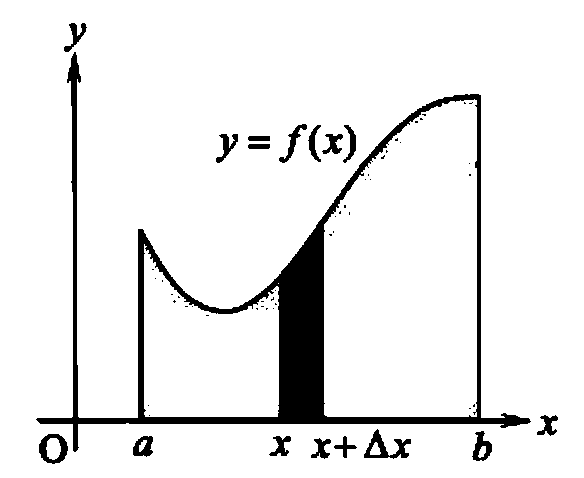
\includegraphics[scale=0.3]{assets/28-8.png}
    \end{center}

    Summing up the approximated area of all the smaller curved trapezoid, then find
    the limit of the sum when $\Delta x \to 0$, we can get the area of the original
    curved trapezoid, i.e.
    \begin{cequation}
        \sum\Delta A \approx \sum f(x)\Delta x\ \xrightarrow{\ \ \ \ \Delta x \to 0\ \ \ \ } \int_a^b f(x)dx
    \end{cequation}

    \begin{center}
        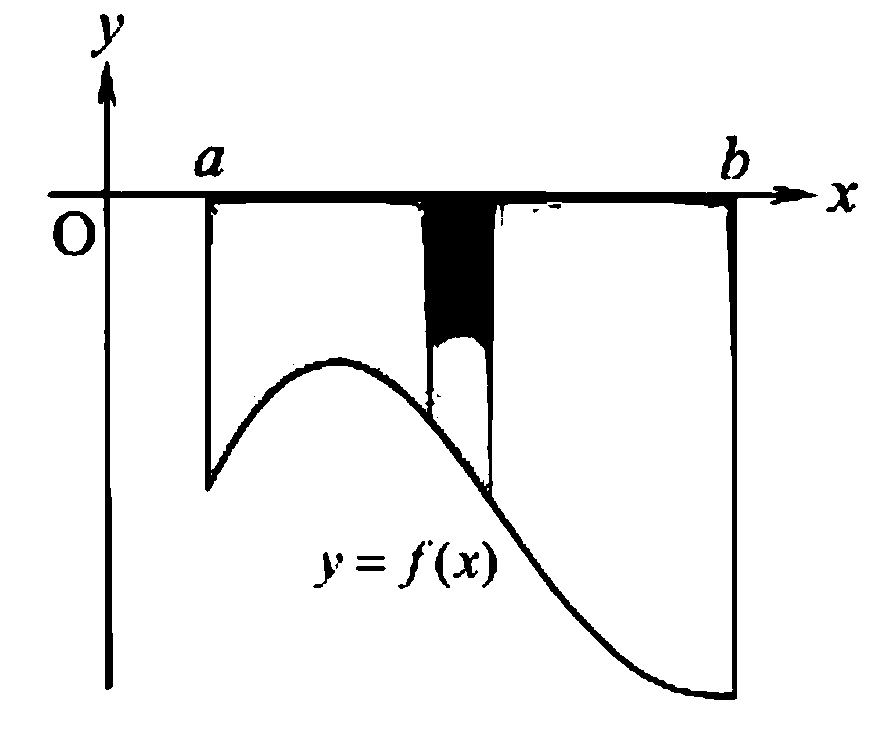
\includegraphics[scale=0.2]{assets/28-9.png}
    \end{center}
    The same can be applied if $f(x) \leq 0$ in the interval $a \leq x \leq b$, as
    shown in the diagram above. The area of the curved trapezoid bounded by the
    curve $y = f(x)$, the lines $x = a$ and $x = b$, the $x$-axis, and the $y$-axis
    is given by
    \begin{cequation}
        A = -\int_a^b f(x)dx
    \end{cequation}

    \begin{center}
        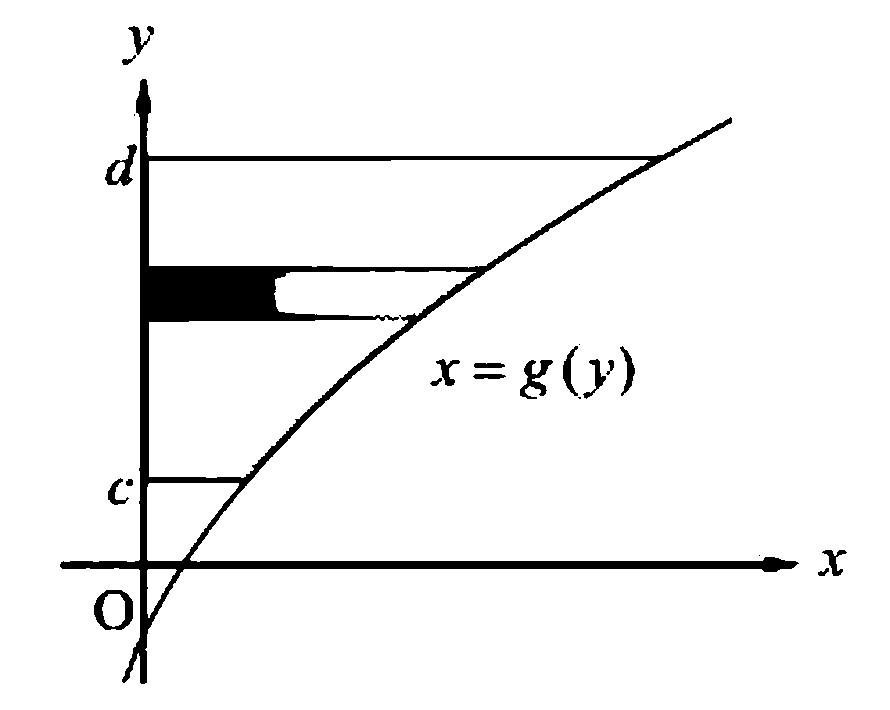
\includegraphics[scale=0.2]{assets/28-10.png}
    \end{center}
    If the target area $A$ is bounded by the lines $y = c$, $y = d$, the $y$-axis,
    and the curve $x = f(y)$, where $f(y) \geq 0$ in the interval $c \leq y \leq
d$, as shown in the diagram above, using the same concept, we can get the area
    of the region
    \begin{cequation}
        A = \int_c^d f(y)dy
    \end{cequation}

    \subsection{Practice 5}
Find the following indefinite integral:
\begin{enumerate}
    \begin{multicols}{2}
        \item $\displaystyle\int\sin2x\cos2x dx$
        \sol{}
        \begin{flalign*}
            I & = \dfrac{1}{2}\int\sin4x dx & \\
              & = -\dfrac{1}{8}\cos4x + C
        \end{flalign*}
        \vfill{}\null{}

        \item $\displaystyle\int\cos^2 2x dx$
        \sol{}
        \begin{flalign*}
            I & = \int\dfrac{1 + \cos 4x}{2} dx                    & \\
              & = \dfrac{1}{2}\int dx + \dfrac{1}{2}\int\cos 4x dx & \\
              & = \dfrac{1}{2}x + \dfrac{1}{8}\sin 4x + C
        \end{flalign*}
    \end{multicols}
    \begin{multicols}{2}
        \item $\displaystyle\int\sin^3 x dx$
        \sol{}
        \begin{flalign*}
            I & = \int\sin^2 x\sin x dx                 & \\
              & = \int(1 - \cos^2 x)\sin x dx           & \\
              & = \int\sin x dx - \int\cos^2 x\sin x dx
        \end{flalign*}
        Let $u = \cos x$, $du = -\sin xdx$.
        \begin{flalign*}
            I & = -\int \cos x dx + \int u^2 du    & \\
              & = -\sin x + \dfrac{1}{3}u^3 + C    & \\
              & = \dfrac{1}{3}\cos^3 x -\sin x + C
        \end{flalign*}

        \item $\displaystyle\int\cos^3 x dx$
        \sol{}
        \begin{flalign*}
            I & = \int\cos^2 x\cos x dx                 & \\
              & = \int(1 - \sin^2 x)\cos x dx           & \\
              & = \int\cos x dx - \int\sin^2 x\cos x dx
        \end{flalign*}
        Let $u = \sin x$, $du = \cos xdx$.
        \begin{flalign*}
            I & = \int \cos x dx - \int u^2 du      & \\
              & = \sin x - \dfrac{1}{3}u^3 + C      & \\
              & = \sin x - \dfrac{1}{3}\sin^3 x + C
        \end{flalign*}
    \end{multicols}
    \begin{multicols}{2}
        \item $\displaystyle\int\tan^4 x\sec^2 x dx$
        \sol{}

        Let $u = \tan x$, $du = \sec^2 xdx$.
        \begin{flalign*}
            I & = \int u^4 du              & \\
              & = \dfrac{u^5}{5} + C       & \\
              & = \dfrac{1}{5}\tan^5 x + C
        \end{flalign*}
        \vfill{}\null{}
        \columnbreak
        \item $\displaystyle\int\tan^4\dfrac{x}{2} dx$
        \sol{}
        \begin{flalign*}
            I & = \int\tan^2\dfrac{x}{2}\tan^2\dfrac{x}{2} dx                             & \\
              & = \int\left(\sec^2\dfrac{x}{2} - 1\right)\tan^2\dfrac{x}{2} dx            & \\
              & = \int\sec^2\dfrac{x}{2}\tan^2\dfrac{x}{2} dx - \int\tan^2\dfrac{x}{2} dx
        \end{flalign*}
        Let $u = \tan\dfrac{x}{2}$, $du = \dfrac{1}{2}\sec^2\dfrac{x}{2}dx$.
        \begin{flalign*}
            I & = 2\int u^2 du - \int \tan^2\dfrac{x}{2} dx                     & \\
              & = \dfrac{2u^3}{3} - \int \left(\sec^2\dfrac{x}{2} - 1\right) dx & \\
              & = \dfrac{2u^3}{3} - \int \sec^2\dfrac{x}{2} dx + \int dx        & \\
              & = \dfrac{2}{3}\tan^3\dfrac{x}{2} - 2\tan\dfrac{x}{2} + x + C
        \end{flalign*}
    \end{multicols}
\end{enumerate}

    \newpage
    If, in the internal $a \leq x \leq b$, $f_2(x) \geq f_1(x) \geq 0$, then the
    area of the region bounded by the curve $y = f_1(x)$, $y = f_2(x)$, the lines
$x = a$ and $x = b$ can be found using definite integrals.
    \begin{center}
        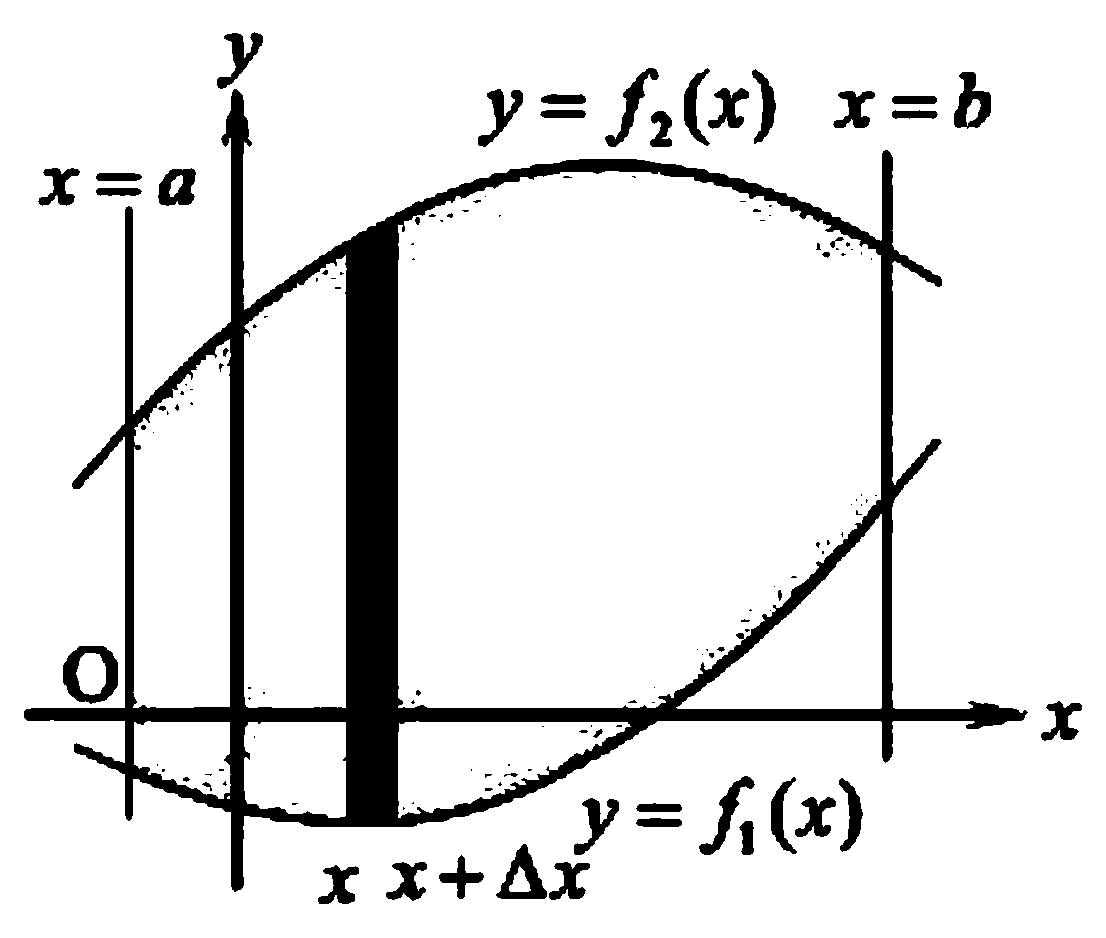
\includegraphics[scale=0.15]{assets/28-16.png}
    \end{center}

    As shown in the diagram above, split the interval $a \leq x \leq b$ into
    multiple smaller intervals. Take any one of the smaller intervals, and express
    it as $[x, x + \Delta x]$. The region in this smaller interval can be
    approximated by a rectangle with width of $\Delta x$ and height of the function
    value $f_2(x) - f_1(x)$, i.e.
    \begin{cequation}
        \Delta A \approx [f_2(x) - f_1(x)]\Delta x
    \end{cequation}

    Summing up the approximated area of all the smaller intervals, then find the
    limit of the sum when $\Delta x \to 0$, we can get the area of the region
    bounded by the curve $y = f_1(x)$, $y = f_2(x)$, the lines $x = a$ and $x = b$,
    i.e.
    \begin{center}
        \framebox{

        \parbox[t][1.3cm]{5cm}{ \addvspace{0.2cm} \centering $\displaystyle A = \int_a^b
            [f_2(x) - f_1(x)]dx$ }}
    \end{center}

    \begin{center}
        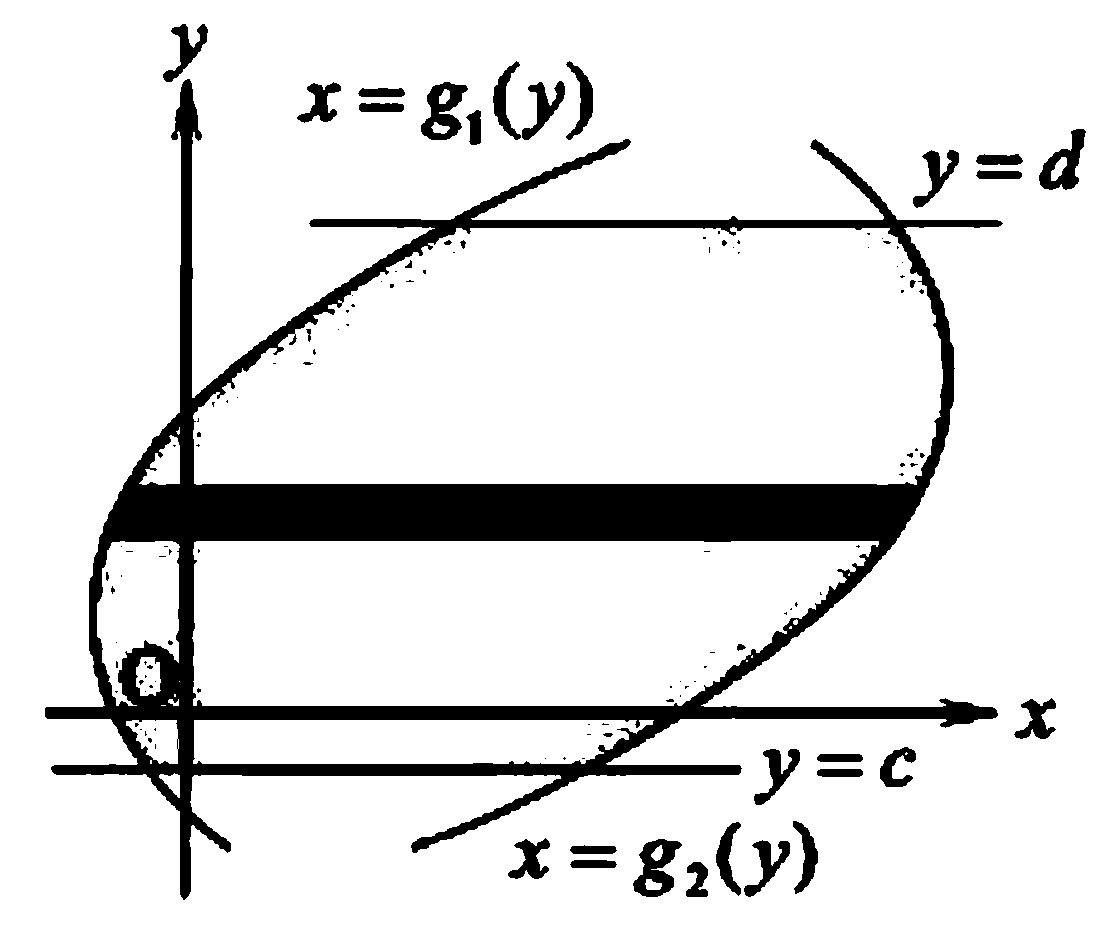
\includegraphics[scale=0.15]{assets/28-17.png}
    \end{center}

    Similarly, if, in the internal $c \leq y \leq d$, $g_2(y) \geq g_1(y) \geq 0$,
    then the area of the region bounded by the curve $x = g_1(y)$, $x = g_2(y)$,
    the lines $y = c$ and $y = d$ is given by
    \begin{center}
        \framebox{

        \parbox[t][1.3cm]{5cm}{ \addvspace{0.2cm} \centering $\displaystyle A = \int_c^d
            [g_2(y) - g_1(y)]dy$ }}
    \end{center}
    Note that when using these formulas, the function $f_2(x)$ must always be greater than or equal to $f_1(x)$ in the interval $[a, b]$.

    \newpage
    \subsection{Practice 6}

Sketch the graph of the function $f(x) = x^3 - 3x^2 + 2$.

    \subsection{Exercise 28.3}

\noindent \hspace{1.2em}\textit{Find the area of the region bounded by the following curves and lines:}
\begin{enumerate}
      \begin{multicols}{2}
            \item $y=3 x^2, x=2, x=5$, and $x$-axis
            \sol{}
            \begin{flalign*}
                  A & = \int_2^5 3x^2 d x    & \\
                    & = \left[x^3\right]_2^5 & \\
                    & = 125 - 8              & \\
                    & = 117
            \end{flalign*}

            \item $y=(x-1)^2, x=4, x$-axis, and $y$-axis
            \sol{}
            \begin{flalign*}
                  A & = \int_0^4 (x-1)^2 d x                 & \\
                    & = \left[\dfrac{1}{3}(x-1)^3\right]_0^4 & \\
                    & = \dfrac{1}{3}(3^3 + 1)                & \\
                    & = \dfrac{28}{3}
            \end{flalign*}
      \end{multicols}

      \vfill\null

      \begin{multicols}{2}
            \item $y=x^2+4 x-21$, and $x$-axis
            \begin{flalign*}
                  x^2 + 4x - 21        & = 0 & \\
                  (x + 7)(x - 3)       & = 0 & \\
                  x = -7 \text{ or } x & = 3
            \end{flalign*}
            In the interval $-7 \leq x \leq 3$, $x^2 + 4x - 21 \leq 0$.
            \begin{flalign*}
                  A & = \left|\int_{-7}^3 (x^2 + 4x - 21) d x\right|                       & \\
                    & = \left|\left[\dfrac{1}{3}x^3 + 2x^2 - 21x\right]_{-7}^3\right|      & \\
                    & = \left|9 + 18 - 63 - \left(-\dfrac{343}{3} + 98 + 147\right)\right| & \\
                    & = \dfrac{500}{3}
            \end{flalign*}

            \item $y=e^{2 x}, x=0, x=4$, and $x$-axis
            \sol{}
            \begin{flalign*}
                  A & = \int_0^4 e^{2x} d x                 & \\
                    & = \left[\dfrac{1}{2}e^{2x}\right]_0^4 & \\
                    & = \dfrac{1}{2}(e^8 - 1)
            \end{flalign*}
      \end{multicols}

      \vfill\null

      \begin{multicols}{2}
            \item $y=\sin \dfrac{x}{2}, 0 \leq x \leq 2 \pi$, and $x$-axis
            \sol{}
            \begin{flalign*}
                  A & = \int_0^{2 \pi} \sin \dfrac{x}{2} d x        & \\
                    & = \left[-2 \cos \dfrac{x}{2}\right]_0^{2 \pi} & \\
                    & = 4
            \end{flalign*}
            \vfill\null

            \columnbreak
            \item $y=\cos x, x=2 \pi, x$-axis, and $y$-axis
            \sol{}
            \begin{flalign*}
                  \cos x & = 0                                & \\
                  x      & = \dfrac{\pi}{2}, \dfrac{3 \pi}{2}
            \end{flalign*}
            In the interval $\dfrac{\pi}{2} \leq x \leq \dfrac{3 \pi}{2}$, $\cos x \leq 0$.
            \begin{flalign*}
                  A & = \int_{0}^{\frac{\pi}{2}} \cos x d x + \left|\int_{\frac{\pi}{2}}^{\frac{3 \pi}{2}} \cos x d x\right| + \int_{\frac{3 \pi}{2}}^{2 \pi} \cos x d x        & \\
                    & = \bigg[\sin x\bigg]_0^{\frac{\pi}{2}} + \left|\bigg[\sin x\bigg]_{\frac{\pi}{2}}^{\frac{3 \pi}{2}}\right| + \bigg[\sin x\bigg]_{\frac{3 \pi}{2}}^{2 \pi} & \\
                    & = 1 + 1 + 1 + 1 = 4
            \end{flalign*}
      \end{multicols}

      \newpage
      \begin{multicols}{2}
            \item $x=y^2, y=3$, and $y$-axis
            \sol{}
            \begin{flalign*}
                  A & = \int_0^3 y^2 d y                 & \\
                    & = \left[\dfrac{1}{3}y^3\right]_0^3 & \\
                    & = 9
            \end{flalign*}

            \vfill{}\null{}
            \columnbreak{}
            \item $x=9 y-y^3$, and $y$-axis
            \sol{}
            \begin{flalign*}
                  9y - y^3   & = 0                   & \\
                  y(9 - y^2) & = 0                   & \\
                  y = 0      & \text{ or } y = \pm 3
            \end{flalign*}
            In the interval $-3 \leq y \leq 0$, $9y - y^3 \leq 0$.
            \begin{flalign*}
                  A & = \left|\int_{-3}^0 (9y - y^3) d y\right| + \int_0^3 (9y - y^3) d y                                                       & \\
                    & = \left|\left[\dfrac{9}{2}y^2 - \dfrac{1}{4}y^4\right]_{-3}^0\right| + \left[\dfrac{9}{2}y^2 - \dfrac{1}{4}y^4\right]_0^3 & \\
                    & = \left|- \dfrac{81}{2} + \dfrac{81}{4}\right| + \dfrac{81}{2} - \dfrac{81}{4}                                            & \\
                    & = \dfrac{81}{2}
            \end{flalign*}
      \end{multicols}

      \begin{multicols}{2}
            \item $y=\dfrac{1}{x}, y=\dfrac{1}{2}, y=2$, and $y$-axis
            \sol{}
            \begin{flalign*}
                  A & = \int_{\frac{1}{2}}^2 \dfrac{1}{x} d x & \\
                    & = \bigg[\ln x\bigg]_{\frac{1}{2}}^2     & \\
                    & = \ln 2 - \ln \dfrac{1}{2}              & \\
                    & = 2 \ln 2
            \end{flalign*}

            \item $y^2=x, x=4$, and $x=16$
            \sol{}
            \begin{flalign*}
                  A & = 2 \int_4^{16} \sqrt{x} d x                        & \\
                    & = 2 \left[\dfrac{2}{3}x^{\frac{3}{2}}\right]_4^{16} & \\
                    & = 2 \left(\dfrac{128}{3} - \dfrac{16}{3}\right)     & \\
                    & = \dfrac{224}{3}
            \end{flalign*}
            \vfill{}\null{}
      \end{multicols}

      \begin{multicols}{2}
            \item Find the area of the region bounded by the curve \\$y=x^2-4$ and the line $y=3
            x$. \sol{}
                  \begin{flalign*}
                        x^2 - 4             & = 3x & \\
                        x^2 - 3x - 4        & = 0  & \\
                        (x - 4)(x + 1)      & = 0  & \\
                        x = 4 \text{ or } x & = -1
                  \end{flalign*}
                  In the interval $-1 \leq x \leq 4$, $x^2 - 4 \leq 3x$.
                  \begin{flalign*}
                        A & = \int_{-1}^4 (3x - x^2 + 4) d x                             & \\
                          & = \left[\dfrac{3}{2}x^2 - \dfrac{1}{3}x^3 + 4x\right]_{-1}^4 & \\
                          & = 24 - \dfrac{64}{3} + 16 - \dfrac{3}{2} - \dfrac{1}{3} + 4  & \\
                          & = \dfrac{125}{6}
                  \end{flalign*}
                  \item Find the area of the region bounded by the curve $y=x^2+2 x$ and the curve
            $y=12+4 x-x^2$.
                  \begin{flalign*}
                        x^2 + 2x            & = 12 + 4x - x^2 & \\
                        2x^2 - 2x - 12      & = 0             & \\
                        (x - 3)(2x + 4)     & = 0             & \\
                        x = 3 \text{ or } x & = -2
                  \end{flalign*}
                  In the interval $-2 \leq x \leq 3$, $x^2 + 2x \leq 12 + 4x - x^2$.
            \begin{flalign*}
                  A & = \int_{-2}^3 (12 + 4x - x^2 - x^2 - 2x) d x      & \\
                    & = \int_{-2}^3 (12 + 2x - 2x^2) d x                & \\
                    & = \left[12x + x^2 - \dfrac{2}{3}x^3\right]_{-2}^3 & \\
                    & = 36 + 9 - 18 + 24 - 4 - \dfrac{16}{3}            & \\
                    & = \dfrac{125}{3}
            \end{flalign*}
      \end{multicols}

      \begin{multicols}{2}
            \item Find the area of the region bounded by the curve $y=\sin x$ and $y=-2 \sin x$
            in the interval $0 \leq x \leq \pi$. \sol{}
            \begin{flalign*}
                  \sin x & = -2 \sin x & \\
                  \sin x & = 0         & \\
                  x      & = 0, \pi
            \end{flalign*}
            In the interval $0 \leq x \leq \pi$, $-2 \sin x \leq \sin x$.
            \begin{flalign*}
                  A & = \int_0^{\pi} (3 \sin x) d x   & \\
                    & = \bigg[-3 \cos x\bigg]_0^{\pi} & \\
                    & = 3 - (-3) = 6
            \end{flalign*}
            \vfill{}\null{}

            \item Find the area of the region bounded by the curve $y=e^x, y=e^{-2 x}$ and the
            lines $x=-2$ and $x=4$. \sol{}
            \begin{flalign*}
                  e^x & = e^{-2x} & \\
                  x   & = 0
            \end{flalign*}
            In the interval $-2 \leq x \leq 0$, $e^x \leq e^{-2x}$.

            In the interval $0 \leq x \leq 4$, $e^{-2x} \leq e^x$.
            \begin{flalign*}
                  A & = \int_{-2}^0 (e^{-2x} - e^x) d x + \int_0^4 (e^x - e^{-2x}) d x                               & \\
                    & = \left[-\dfrac{1}{2}e^{-2x} - e^x\right]_{-2}^0 + \left[e^x + \dfrac{1}{2}e^{-2x}\right]_0^4  & \\
                    & = -\dfrac{1}{2} - 1 + \dfrac{1}{2}e^{4} + e^{-2} + e^4 + \dfrac{1}{2}e^{-8} - 1 - \dfrac{1}{2} & \\
                    & = \dfrac{3}{2}e^4 + e^{-2} + \dfrac{1}{2}e^{-8} - 3
            \end{flalign*}
      \end{multicols}

      \vfill\null

      \item Find the area of the region bounded by the curve $y=x^3-10 x^2+28 x$ and the
            line $y=4 x$. \sol{}
            \begin{flalign*}
                  x^3 - 10x^2 + 28x   & = 4x                  & \\
                  x^3 - 10x^2 + 24x   & = 0                   & \\
                  x(x^2 - 10x + 24)   & = 0                   & \\
                  x = 0 \text{ or } x & = 4 \text{ or } x = 6
            \end{flalign*}
            In the interval $0 \leq x \leq 4$, $x^3 - 10x^2 + 28x \geq 4x$.

            In the interval $4 \leq x \leq 6$, $x^3 - 10x^2 + 28x \leq 4x$.
            \begin{flalign*}
                  A & = \int_0^4 (x^3 - 10x^2 + 28x - 4x) d x + \int_4^6 (4x - x^3 + 10x^2 - 28x) d x                                              & \\
                    & = \int_0^4 (x^3 - 10x^2 + 24x) d x + \int_4^6 (-x^3 + 10x^2 - 24x) d x                                                       & \\
                    & = \left[\dfrac{1}{4}x^4 - \dfrac{10}{3}x^3 + 12x^2\right]_0^4 + \left[-\dfrac{1}{4}x^4 + \dfrac{10}{3}x^3 - 12x^2\right]_4^6 & \\
                    & = 64 - \dfrac{640}{3} + 192 - 324 + 720 - 432 + 64 - \dfrac{640}{3} + 192                                                    & \\
                    & = \dfrac{148}{3}
            \end{flalign*}
            \vfill\null

            \newpage

      \item Find the area of the region bounded by the curve $x=8 y-y^2, x=16 y-y^2-48$,
            and $y$-axis. \sol{}
            \begin{flalign*}
                  8y - y^2 & = 16y - y^2 - 48 & \\
                  8y       & = 48             & \\
                  y        & = 6
            \end{flalign*}

      \item Find the area of the region bounded by the curve $x=2 y^2-8 y+10$ and
            $x=y^2-y$.
      \item Given that the curve $y=f(x)$ passes through point $(1,0)$, and the gradient of
            any point on the curve $(x, y)$ is $3 x^2-3$. Find the area of the region
            bounded by the curve, $x=2$ and $x$.
\end{enumerate}

    \newpage
    \section{Volume of Revolution}
    The solid formed by rotating a flat surface around a certain straight line on
    the surface is called the \textbf{solid of revolution}, for example the right
    cylinder, right cone, and sphere.

    \begin{center}
        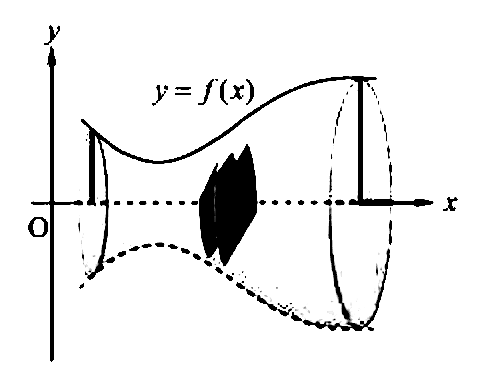
\includegraphics[scale=0.3]{assets/28-22a.png}
    \end{center}

    The diagram above shows a solid of revolution formed by rotating the area
    bounded by the curve $y = f(x)$, the lines $x = a$, $x = b$, and the $x$-axis
    around the $x$-axis. We can utilize the methods discussed in the last section
    to find the volume of this solid of revolution.

    \vspace{0.5cm}
    \begin{vwcol}[widths={0.7,0.3},justify=flush,rule=0pt,indent=1em]

        Split the interval $a \leq x \leq b$ into multiple smaller intervals. Take any
        one of the smaller intervals, and express it as $[x, x + \Delta x]$. The region
        in this smaller interval can be approximated by a rectangle with width of
        $\Delta x$ and height of the function value $f(x)$. Rotate this rectangle
        around the $x$-axis, we get a cylinder with radius $f(x)$ and height $\Delta
            x$, as shown in the diagram on the right-hand side. Hence, the approximated
        volume of the solid of revolution in this smaller interval is
        \begin{cequation}
            \Delta V \approx \pi[f(x)]^2\Delta x
        \end{cequation}

        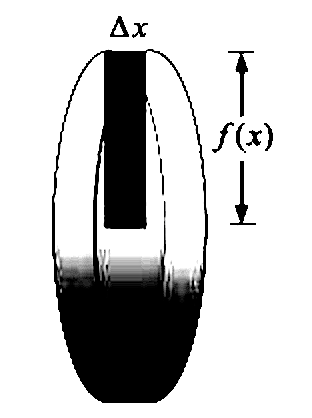
\includegraphics[scale=0.3]{assets/28-22b.png}
    \end{vwcol}
    \vspace{0.5cm}
    Summing up the approximated volume of all the smaller intervals, then find the
    limit of the sum when $\Delta x \to 0$, we can get the volume of the solid of
    revolution, i.e.
    \begin{center}
        \framebox{

        \parbox[t][1.3cm]{4cm}{ \addvspace{0.2cm} \centering $\displaystyle V =
            \pi\int_a^b[f(x)]^2dx$ }}
    \end{center}
    \begin{center}
        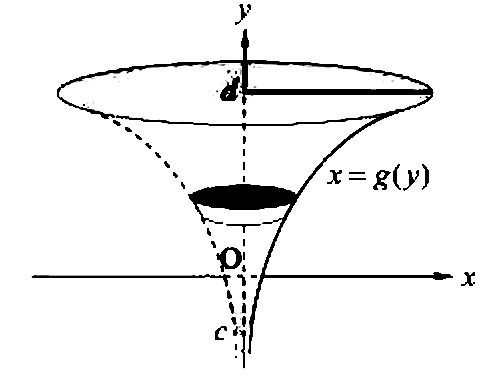
\includegraphics[scale=0.3]{assets/28-23.png}
    \end{center}

    Similarly, if the solid of revolution is formed by rotating the area bounded by
    the curve $x = g(y)$, the lines $y = c$, $y = d$, and the $y$-axis around the
$y$-axis, then the volume of the solid of revolution is given by
    \begin{center}
        \framebox{

        \parbox[t][1.3cm]{4cm}{ \addvspace{0.2cm} \centering $\displaystyle V =
            \pi\int_c^d[g(y)]^2dy$ }}
    \end{center}

    \newpage
    \subsection{Practice 7}
\begin{enumerate}
      \begin{multicols}{2}
            \item A drop of ink gradually spread after being dropped onto a piece of paper. At
            $t$ seconds, its area is $A = \left(3t^2 + \dfrac{1}{5}t + 2\right)$mm$^2$.
            Find the rate of change of the ink spread at $t = 2$ second. \sol{}
            \begin{flalign*}
                  \dfrac{dA}{dt} & = 6t + \dfrac{1}{5}
            \end{flalign*}
            When $t = 2$,
            \begin{flalign*}
                  \dfrac{dA}{dt} & = 6(2) + \dfrac{1}{5}      \\
                                 & = 12 + \dfrac{1}{5}        \\
                                 & = \dfrac{61}{5}            \\
                                 & = 12.2\text{mm}^2\text{/s}
            \end{flalign*}
            \vfill\null

            \item The radius of a sphere increases at a rate of $3$cm/s. When the radius is
            $5$cm, find the rate of change of the surface area of the sphere. \sol{}
            \begin{flalign*}
                  \dfrac{dr}{dt} & = 3\text{cm/s}                      \\
                  A              & = 4\pi r^2                          \\
                  \dfrac{dA}{dr} & = 8\pi r                            \\
                  \dfrac{dA}{dt} & = \dfrac{dA}{dr}\cdot\dfrac{dr}{dt} \\
                                 & = 8\pi r\cdot 3\text{cm/s}          \\
                                 & = 24\pi r\text{cm}^2\text{/s}
            \end{flalign*}
            When $r = 5$,
            \begin{flalign*}
                  \dfrac{dA}{dt} & = 24\pi(5)\text{cm}^2\text{/s} \\
                                 & = 120\pi\text{cm}^2\text{/s}
            \end{flalign*}
      \end{multicols}
\end{enumerate}

    If a region is bounded by the curve $y = f_1(x)$, $y = f_2(x)$, the lines $x =
a$, $x = b$, and the $x$-axis, and $f_2 \geq f_1 \geq 0$, then the volume of
    the solid of revolution formed by rotating this region around the $x$-axis, as
    shown in the diagram below, is given by
    \begin{center}
        \framebox{

        \parbox[t][1.3cm]{12cm}{ \addvspace{0.2cm} \centering $\displaystyle V =
            \pi\int_a^b[f_2(x)]^2dx - \pi\int_a^b[f_1(x)]^2dx =
            \pi\int_a^b\left\{[f_2(x)]^2 - [f_1(x)]^2\right\}dx$ }}
    \end{center}
    \begin{center}
        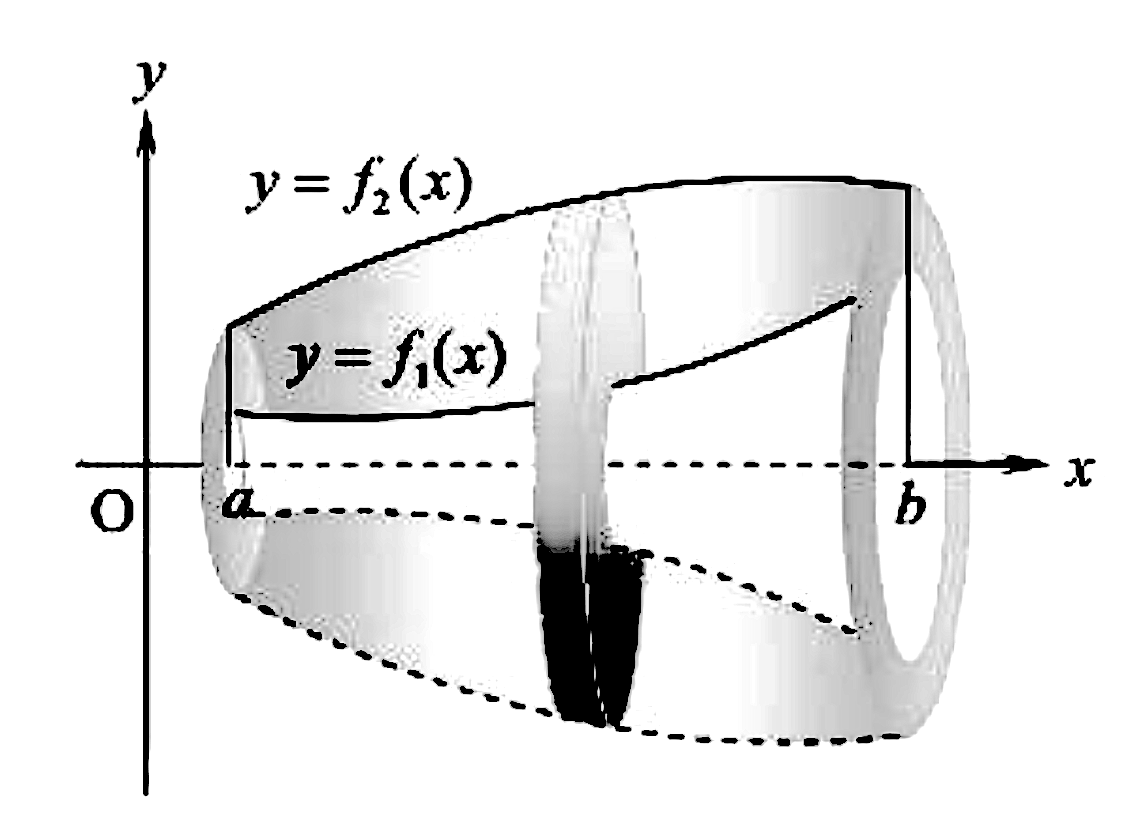
\includegraphics[scale=0.15]{assets/28-29.png}
    \end{center}

    Similarly, if a region is bounded by the curve $x = g_1(y)$, $x = g_2(y)$, the
    lines $y = c$, $y = d$, and the $y$-axis, and $g_2 \geq g_1 \geq 0$, then the
    volume of the solid of revolution formed by rotating this region around the
$y$-axis, as shown in the diagram below, is given by \vspace{-0.9em}
\begin{center}
    \framebox{

    \parbox[t][1.3cm]{6cm}{ \addvspace{0.2cm} \centering $\displaystyle V =
        \pi\int_c^d\left\{[g_2(y)]^2 - [g_1(y)]^2\right\}dy$ }}
\end{center}
\begin{center}
    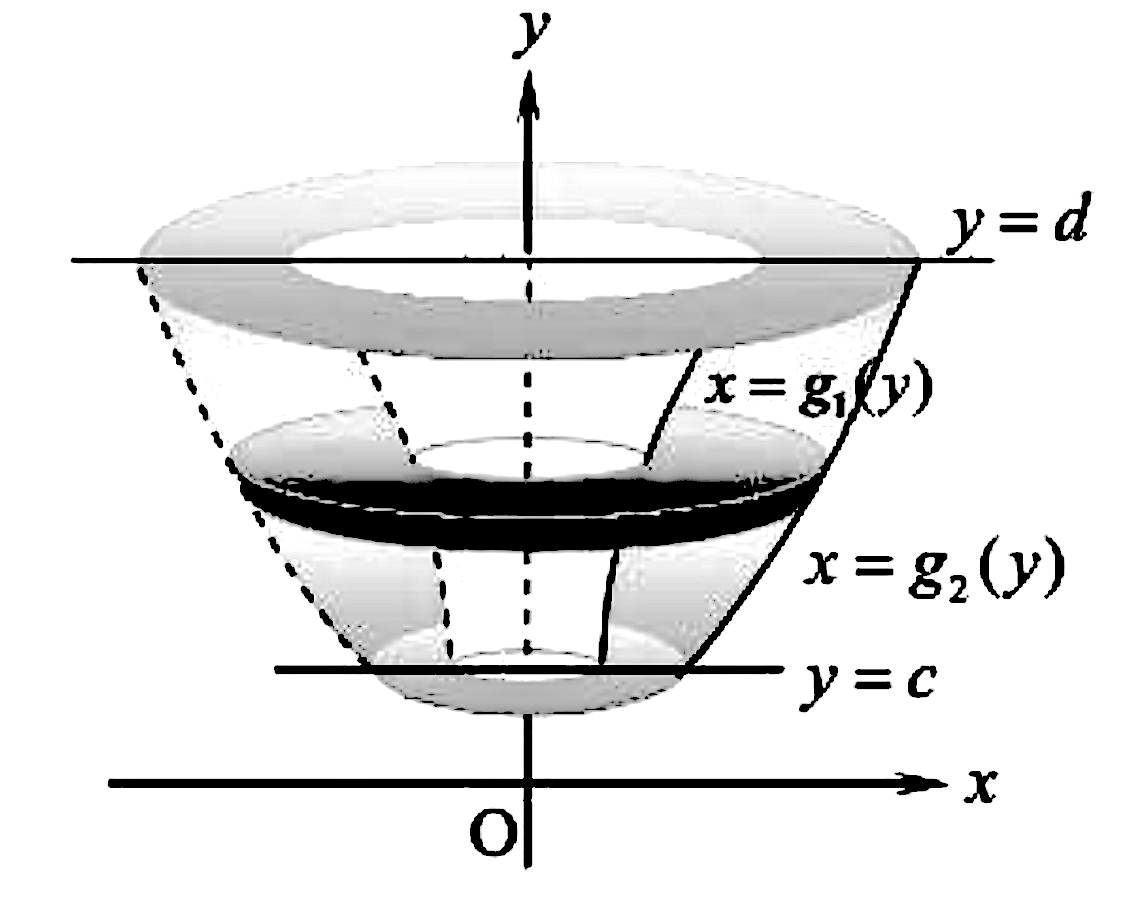
\includegraphics[scale=0.15]{assets/28-30.png}
\end{center}

\subsection{Practice 8}

\begin{enumerate}
      \item The side length of a cube increases from 1cm to $1.01$cm, how much does its
            surface area increase approximately? \sol{}

            Let the side length be $x$cm, then the surface area is $A = 6x^2$.
            \begin{flalign*}
                  \dfrac{dA}{dx}             & = 12x                  & \\
                  \dfrac{\Delta A}{\Delta x} & \approx \dfrac{dA}{dx} & \\
                  \Delta A                   & \approx 12x\Delta x
            \end{flalign*}
            \vspace{-0.8em}
            When $x = 1$cm, $\Delta x = 0.01$cm,
            \begin{flalign*}
                  \Delta A & \approx 12(1)(0.01) = 0.12\text{cm}^2 &
            \end{flalign*}
            $\therefore$ The surface area increases by $0.12$cm$^2$ approximately.

            \begin{multicols}{2}
                  \item After a metal ball was heated, its radius had increased form 4cm to $4.01$cm.
                  Find the approximate increment of its volume and surface area. \sol{}

                  Let the radius be $r$cm, then the volume is $V = \dfrac{4}{3}\pi r^3$ and the
                  surface area is $A = 4\pi r^2$.
                  \begin{flalign*}
                        \dfrac{dV}{dr}             & = 4\pi r^2               & \\
                        \dfrac{dA}{dr}             & = 8\pi r                 & \\
                        \dfrac{\Delta V}{\Delta r} & \approx \dfrac{dV}{dr}   & \\
                        \Delta V                   & \approx 4\pi r^2\Delta r & \\
                        \dfrac{\Delta A}{\Delta r} & \approx \dfrac{dA}{dr}   & \\
                        \Delta A                   & \approx 8\pi r\Delta r
                  \end{flalign*}
                  When $r = 4$cm, $\Delta r = 0.01$cm,
                  \begin{flalign*}
                        \Delta V & \approx 4\pi(4)^2(0.01) & \\
                                 & = 0.64\pi\text{cm}^3    & \\
                        \Delta A & \approx 8\pi(4)(0.01)   & \\
                                 & = 0.32\pi\text{cm}^2
                  \end{flalign*}
                  $\therefore$ The volume increases by $0.64\pi$cm$^3$ and the surface area increases by $0.32\pi$cm$^2$ approximately.
                  \columnbreak
                  \item Find the approximate value of $\sqrt{15}$. \sol{}
                  \begin{flalign*}
                        f(x)                       & = \sqrt{x}                           & \\
                        f'(x)                      & = \dfrac{1}{2\sqrt{x}}               & \\
                        \dfrac{\Delta f}{\Delta x} & \approx \dfrac{df}{dx}               & \\
                        \Delta f                   & \approx \dfrac{1}{2\sqrt{x}}\Delta x
                  \end{flalign*}
                  When $x = 16$, $\Delta x = -1$,
                  \begin{flalign*}
                        \Delta f & \approx \dfrac{1}{2\sqrt{16}}(-1) & \\
                                 & = -\dfrac{1}{8}                   & \\
                                 & = -0.125
                  \end{flalign*}
                  $\therefore$ $\sqrt{15} \approx \sqrt{16} - 0.125 = 3.875$.
            \end{multicols}
\end{enumerate}



\subsection{Exercise 28.4}

\noindent \hspace{1.2em}\textit{Find the volume of the solid of revolution formed by rotating the regions bounded by the following curves and lines about the $x$-axis (Question 1 to 7):}

\begin{enumerate}
      \begin{multicols}{2}
            \item $y=\sqrt{x}, x=4, x=9$, and $x$-axis
            \sol{}
            \begin{flalign*}
                  V_x & = \int_{4}^{9} \pi \left( \sqrt{x} \right)^2 dx & \\
                      & = \pi \int_{4}^{9} x dx                         & \\
                      & = \pi \left[ \frac{x^2}{2} \right]_{4}^{9}      & \\
                      & = \pi \left( \frac{81}{2} - 8 \right)           & \\
                      & = \frac{65 \pi}{2}
            \end{flalign*}

            \item $y=3 x, x=4$, and $x$-axis
            \sol{}
            \begin{flalign*}
                  V_x & = \int_{0}^{4} \pi \left( 3 x \right)^2 dx & \\
                      & = \pi \int_{0}^{4} 9 x^2 dx                & \\
                      & = \pi \left[ 3 x^3 \right]_{0}^{4}         & \\
                      & = 192 \pi
            \end{flalign*}
      \end{multicols}

      \begin{multicols}{2}
            \item $y=x(x-2)$, and $x$-axis
            \sol{}
            \begin{flalign*}
                  V_x & = \pi \int_{0}^{2} x^2 (x-2)^2 dx                                 & \\
                      & = \pi \int_{0}^{2} x^2 (x^2 - 4x + 4) dx                          & \\
                      & = \pi \int_{0}^{2} x^4 - 4x^3 + 4x^2 dx                           & \\
                      & = \pi \left[ \frac{x^5}{5} - x^4 + \frac{4x^3}{3} \right]_{0}^{2} & \\
                      & = \pi\left[\dfrac{32}{5} - 16 + \dfrac{32}{3}\right]              & \\
                      & = \dfrac{16 \pi}{15}
            \end{flalign*}

            \item $x^2+y^2=4, x=0$, and $x=2$
            \sol{}
            \begin{flalign*}
                  V_x & = \pi \int_{0}^{2} \left( 4 - x^2 \right) dx    & \\
                      & = \pi \left[ 4x - \frac{x^3}{3} \right]_{0}^{2} & \\
                      & = \frac{16 \pi}{3}
            \end{flalign*}
      \end{multicols}

      \begin{multicols}{2}
            \item $y=\sin x, x=0, x=\pi$, and $x$-axis
            \sol{}
            \begin{flalign*}
                  V_x & = \pi \int_{0}^{\pi} \sin^2 x dx                               & \\
                      & = \pi \int_{0}^{\pi} \frac{1 - \cos 2x}{2} dx                  & \\
                      & = \frac{\pi}{2} \int_{0}^{\pi} (1 - \cos 2x) dx                & \\
                      & = \frac{\pi}{2} \left[ x - \frac{\sin 2x}{2} \right]_{0}^{\pi} & \\
                      & = \frac{\pi}{2} \left( \pi - 0 \right)                         & \\
                      & = \frac{\pi^2}{2}
            \end{flalign*}

            \item $y=e^x, x=-1, x=1$, and $x$-axis
            \sol{}
            \begin{flalign*}
                  V_x & = \pi \int_{-1}^{1} e^{2x} dx                         & \\
                      & = \pi \left[ \frac{e^{2x}}{2} \right]_{-1}^{1}        & \\
                      & = \pi \left( \frac{e^2}{2} - \frac{e^{-2}}{2} \right) & \\
                      & = \frac{\pi}{2} \left( e^2 - e^{-2} \right)
            \end{flalign*}
      \end{multicols}

      \newpage
      \item $y=x^3+x^2-2 x$, and $x$-axis
            \sol{}
            \begin{flalign*}
                  V_x & = \pi \int_{-2}^{1} \left( x^3 + x^2 - 2 x \right)^2 dx                                                                                                  & \\
                      & = \pi \int_{-2}^{1} (x^6 + x^4 + 4x^2 + 2x^5 - 4x^3 - 4x^4) dx                                                                                           & \\
                      & = \pi \int_{-2}^{1} (x^6 + 2x^5 - 3x^4 - 4x^3 + 4x^2) dx                                                                                                 & \\
                      & = \pi \left[ \frac{x^7}{7} + \frac{x^6}{3} - \dfrac{3}{5}x^5 - x^4 + \frac{4x^3}{3} \right]_{-2}^{1}                                                     & \\
                      & = \pi \left( \dfrac{1}{7} + \dfrac{1}{3} - \dfrac{3}{5} - 1 + \dfrac{4}{3} + \dfrac{128}{7} - \dfrac{64}{3} - \dfrac{96}{5} + 16 + \dfrac{32}{3} \right) & \\
                      & = \dfrac{162}{35} \pi
            \end{flalign*}
\end{enumerate}

\noindent \hspace{1.2em}\textit{Find the volume of the solid of revolution formed by rotating the regions bounded by the following curves and lines about the $y$-axis (Question 8 to 14):}

\begin{enumerate}[resume]
      \begin{multicols}{2}
            \item $y=x^3, y=8$, and $y$-axis
            \sol{}
            \begin{flalign*}
                  V_y & = \pi \int_{0}^{8} \left( \sqrt[3]{y} \right)^2 dy       & \\
                      & = \pi \int_{0}^{8} y^{\frac{2}{3}} dy                    & \\
                      & = \pi \left[ \frac{3}{5} y^{\frac{5}{3}} \right]_{0}^{8} & \\
                      & = \frac{3 \pi}{5} \left( 8^{\frac{5}{3}} - 0 \right)     & \\
                      & = \frac{96 \pi}{5}
            \end{flalign*}

            \item $x=\sqrt{y-1}, y=4$, and $y$-axis
            \sol{}
            \begin{flalign*}
                  V_y & = \pi \int_{1}^{4} \left( \sqrt{y-1} \right)^2 dy & \\
                      & = \pi \int_{1}^{4} (y-1) dy                       & \\
                      & = \pi \left[ \frac{y^2}{2} - y \right]_{1}^{4}    & \\
                      & = \pi \left( 8 - 4 - \frac{1}{2} + 1 \right)      & \\
                      & = \frac{9 \pi}{2}
            \end{flalign*}
      \end{multicols}

      \begin{multicols}{2}
            \item $y^2=x+3, y=2, x$-axis, and $y$-axis
            \sol{}
            \begin{flalign*}
                  V_y & = \pi \int_{0}^{2} \left( y^2 - 3 \right)^2 dy           & \\
                      & = \pi \int_{0}^{2} (y^4 - 6 y^2 + 9) dy                  & \\
                      & = \pi \left[ \frac{y^5}{5} - 2 y^3 + 9 y \right]_{0}^{2} & \\
                      & = \pi \left( \frac{32}{5} - 16 + 18 \right)              & \\
                      & = \frac{42 \pi}{5}
            \end{flalign*}

            \item $y^2=x+1$, and $y$-axis
            \sol{}
            \begin{flalign*}
                  V_y & = \pi \int_{-1}^{1} \left( y^2 - 1 \right)^2 dy                                    & \\
                      & = \pi \int_{-1}^{1} (y^4 - 2 y^2 + 1) dy                                           & \\
                      & = \pi \left[ \frac{y^5}{5} - \frac{2 y^3}{3} + y \right]_{-1}^{1}                  & \\
                      & = \pi \left( \frac{1}{5} - \frac{2}{3} + 1 + \frac{1}{5} - \frac{2}{3} + 1 \right) & \\
                      & = \frac{16 \pi}{15}
            \end{flalign*}
      \end{multicols}

      \newpage
      \begin{multicols}{2}
            \item $x^2-y^2=4, y=3$, and $x$-axis
            \sol{}
            \begin{flalign*}
                  V_x & = \pi \int_{0}^{3} (4+y^2) dy                   & \\
                      & = \pi \left[ 4y + \frac{y^3}{3} \right]_{0}^{3} & \\
                      & = \pi \left( 12 + 9 \right)                     & \\
                      & = 21 \pi
            \end{flalign*}
            \vfill\null

            \item $y=1-\sqrt{x}, x$-axis, and $y$-axis
            \sol{}
            \begin{flalign*}
                  V_x & = \pi \int_{0}^{1} \left( 1 - y \right)^4 dy                       & \\
                      & = \pi \int_{0}^{1} (1 - 4y + 6y^2 - 4y^3 + y^4) dy                 & \\
                      & = \pi \left[ y - 2y^2 + 2y^3 - y^4 + \frac{y^5}{5} \right]_{0}^{1} & \\
                      & = \pi \left( 1 - 2 + 2 - 1 + \frac{1}{5} \right)                   & \\
                      & = \frac{\pi}{5}
            \end{flalign*}
      \end{multicols}

      \item $y=\dfrac{1}{x}-1, y=1, x$-axis, and $y$-axis
            \sol{}
            \begin{flalign*}
                  V_x & = \pi \int_{0}^{1} \frac{1}{(y + 1)^2} dy
            \end{flalign*}
            Let $u = y + 1$, then $du = dy$. When $y = 0$, $u = 1$, when $y = 1$, $u = 2$.
            \begin{flalign*}
                  V_x & = \pi \int_{1}^{2} \frac{1}{u^2} du       & \\
                      & = \pi \left[ -\frac{1}{u} \right]_{1}^{2} & \\
                      & = \pi \left( -\frac{1}{2} + 1 \right)     & \\
                      & = \frac{\pi}{2}
            \end{flalign*}

      \item Given that a region is bounded by the curve $y=4-x^2$ and the $x$-axis. Find
            the volume of the solid of revolution formed by rotating this region about the
            $x$-axis and the $y$-axis respectively. \sol{}
            \begin{flalign*}
                  V_x & = \pi \int_{-2}^{2} (4-x^2)^2 dx                                                         & \\
                      & = \pi \int_{-2}^{2} (16 - 8x^2 + x^4) dx                                                 & \\
                      & = \pi \left[ 16x - \frac{8x^3}{3} + \frac{x^5}{5} \right]_{-2}^{2}                       & \\
                      & = \pi \left( 32 - \frac{64}{3} + \frac{32}{5} + 32 - \frac{64}{3} + \frac{32}{5} \right) & \\
                      & = \frac{512 \pi}{15}
            \end{flalign*}
            \begin{flalign*}
                  V_y & = \pi \int_{0}^{4} \left( 4 - y \right)dy       & \\
                      & = \pi \left[ 4y - \frac{y^2}{2} \right]_{0}^{4} & \\
                      & = \pi \left( 16 - 8 \right)                     & \\
                      & = 8 \pi
            \end{flalign*}

      \item Given that a region is bounded by the curve $y=5-\sqrt{x}, x$-axis, and
            $y$-axis. Find the volume of the solid of revolution formed by rotating this
            region about the $x$-axis and the $y$-axis respectively. \sol{} \vspace{-0.8cm}
            \begin{multicols}{2}
                  \begin{flalign*}
                        V_x & = \pi \int_{0}^{25} \left( 5 - \sqrt{x} \right)^2 dx                            & \\
                            & = \pi \int_{0}^{25} \left(25 - 10 \sqrt{x} + x\right) dx                        & \\
                            & = \pi \left[ 25x - \frac{20x^{\frac{3}{2}}}{3} + \frac{x^2}{2} \right]_{0}^{25} & \\
                            & = \pi \left( 625 - \frac{2500}{3} + \frac{625}{2} \right)                       & \\
                            & = \frac{625 \pi}{6}
                  \end{flalign*}
                  \vfill\null
                  \begin{flalign*}
                        V_y & = \pi \int_{0}^{5} \left( 5 - y \right)^4 dy                              & \\
                            & = \pi \int_{0}^{5} (y^4 - 20y^3 + 150y^2 - 500y + 625) dy                 & \\
                            & = \pi \left[ \frac{y^5}{5} - 5y^4 + 50y^3 - 250y^2 + 625y \right]_{0}^{5} & \\
                            & = \pi \left( 625 - 3125 + 6250 - 6250 + 3125 \right)                      & \\
                            & = 625 \pi
                  \end{flalign*}
                  \vfill\null
            \end{multicols}
            \vfill\null

      \item Find the volume of the solid of revolution formed by rotating the region
            bounded by the cu rve $y^2=9 x$, the line $y=6$, and the $y$-axis about the the
            $y$-axis. \sol{}
            \begin{flalign*}
                  V_y & = \pi \int_{0}^{6} \left( \frac{y^2}{9} \right)^2 dy & \\
                      & = \pi \int_{0}^{6} \frac{y^4}{81} dy                 & \\
                      & = \pi \left[ \frac{y^5}{405} \right]_{0}^{6}         & \\
                      & = \frac{7776 \pi}{405}                               & \\
                      & = \frac{96 \pi}{5}
            \end{flalign*}
            \vfill\null

      \item Given that a region is bounded by the curve $y=x^2+1$, the line $x=-2, x=2$,
            and $x$-axis. Find the volume of the solid of revolution formed by rotating
            this region about the $x$-axis and the $y$-axis respectively. \sol{}
            \vspace{-0.8cm}
            \begin{multicols}{2}
                  \begin{flalign*}
                        V_x & = \pi \int_{-2}^{2} \left( x^2 + 1 \right)^2 dx                                                              & \\
                            & = \pi \int_{-2}^{2} (x^4 + 2x^2 + 1) dx                                                                      & \\
                            & = \pi \left[ \frac{x^5}{5} + \frac{2x^3}{3} + x \right]_{-2}^{2}                                             & \\
                            & = \pi \left( \frac{32}{5} + \frac{16}{3} + 2 + \frac{32}{5} + \frac{16}{3} + 2 \right)  = \frac{412 \pi}{15}
                  \end{flalign*}
                  \vfill\null
                  \begin{flalign*}
                        V_y & = \pi \int_{1}^{5} (y-1) dy + \pi(2)^2\cdot 1                   & \\
                            & = \pi \left[ \frac{y^2}{2} - y \right]_{1}^{5} + 4\pi           & \\
                            & = \pi \left( \frac{25}{2} - 5 - \dfrac{1}{2} + 1\right)  + 4\pi & \\
                            & = 12 \pi
                  \end{flalign*}
                  \vfill\null
            \end{multicols}
            \vfill\null

            \newpage
            \begin{multicols}{2}
                  \item Find the volume of the solid of revolution formed by \\rotating the region
                  bounded by the curve $y=x(6-x)$ \\and the line $y=3 x$ about the $x$-axis.
                  \sol{}
                  \begin{flalign*}
                        V_x & = \pi \int_{0}^{3} \left[x^2(6-x)^2 - (3x)^2\right] dx   & \\
                            & = \pi \int_{0}^{3} (x^4 - 12x^3 + 36x^2 - 9x^2) dx       & \\
                            & = \pi \int_{0}^{3} (x^4 - 12x^3 + 27x^2) dx              & \\
                            & = \pi \left[ \frac{x^5}{5} - 3x^4 + 9x^3 \right]_{0}^{3} & \\
                            & = \pi \left( \frac{243}{5} - 81 + 81 \right)             & \\
                            & = \frac{162 \pi}{5}
                  \end{flalign*}

                  \item Find the volume of the solid of revolution formed by rotating the region
                  bounded by the curve $y=x^2$, the lines $x=1$ and $y=9$ about the $y$-axis.
                  \sol{}
                  \begin{flalign*}
                        V_y & = \pi \int_{1}^{9} y dy - \pi(1)^2 \cdot 8             & \\
                            & = \pi \left[ \frac{y^2}{2} \right]_{1}^{9} - 8\pi      & \\
                            & = \pi \left( \frac{81}{2} - \frac{1}{2} \right) - 8\pi & \\
                            & = \frac{80 \pi}{2} - 8\pi                              & \\
                            & = 32 \pi
                  \end{flalign*}
            \end{multicols}
            \vfill\null

      \item Given that a region is bounded by the curve $y^2=8 x$ and the line $y=2 x$.
            Find the volume of the solid of revolution formed by rotating this region about
            the $x$-axis and the $y$-axis respectively. \sol{} \vspace{-0.8cm}
            \begin{multicols}{2}
                  \begin{flalign*}
                        V_x & = \pi \int_{0}^{2} (8x - 4x^2) dx                  & \\
                            & = \pi \left[ 4x^2 - \frac{4x^3}{3} \right]_{0}^{2} & \\
                            & = \pi \left( 16 - \frac{32}{3} \right)             & \\
                            & = \frac{16 \pi}{3}
                  \end{flalign*}
                  \vfill\null
                  \begin{flalign*}
                        V_y & = \pi \int_{0}^{4} \left( \frac{y^2}{4} - \dfrac{y^4}{64} \right) dy                 & \\
                            & = \dfrac{\pi}{64} \int_{0}^{4} \left( 16y^2 - y^4 \right) dy                         & \\
                            & = \dfrac{\pi}{64} \left[ \frac{16y^3}{3} - \frac{y^5}{5} \right]_{0}^{4}             & \\
                            & = \dfrac{\pi}{64} \left( \frac{1024}{3} - \frac{1024}{5} \right) = \frac{32 \pi}{15}
                  \end{flalign*}
                  \vfill\null
            \end{multicols}
            \vfill\null

      \item Given that a region is bounded by the curve $y^2=8 x$ and $y=8 x^2$. Find the
            volume of the solid of revolution formed by rotating this region about the
            $x$-axis and the $y$-axis respectively. \sol{} \vspace{-0.8cm}
            \begin{multicols}{2}
                  \begin{flalign*}
                        V_x & = \pi \int_{0}^{\frac{1}{2}} (8x - 64x^4) dx                  & \\
                            & = \pi \left[ 4x^2 - \frac{64x^5}{5} \right]_{0}^{\frac{1}{2}} & \\
                            & = \pi \left( 1 - \frac{64}{5} \cdot \frac{1}{32} \right)      & \\
                            & = \frac{3 \pi}{5}
                  \end{flalign*}
                  \vfill\null
                  \begin{flalign*}
                        V_y & = \pi \int_{0}^{2} \left( \frac{y}{8} - \frac{y^4}{64} \right) dy     & \\
                            & = \dfrac{\pi}{64} \int_{0}^{2} \left( 8y - y^4 \right) dy             & \\
                            & = \dfrac{\pi}{64} \left[ 4y^2 - \frac{y^5}{5} \right]_{0}^{2}         & \\
                            & = \dfrac{\pi}{64} \left( 16 - \frac{32}{5} \right) = \frac{3 \pi}{20}
                  \end{flalign*}
                  \vfill\null
            \end{multicols}
            \vfill\null

      \item Given that a region is bounded by the curve $y^2=2 x$ and $y^2=12-4 x$. Find
            the volume of the solid of revolution formed by rotating this region about the
            $x$-axis and the $y$-axis respectively. \sol{} \vspace{-0.8cm}
            \begin{multicols}{2}
                  \begin{flalign*}
                        V_x & = \pi \int_{0}^{2} 2xdx + \pi \int_{2}^{3} (12-4x)dx                     & \\
                            & = \pi \left[ x^2 \right]_{0}^{2} + \pi \left[ 12x - 2x^2 \right]_{2}^{3} & \\
                            & = 4\pi + \pi \left( 36 - 18 - 24 + 8 \right)                             & \\
                            & = 6\pi
                  \end{flalign*}
                  \vfill\null
                  \columnbreak
                  \begin{flalign*}
                        V_y & = \pi \int_{-2}^{2} \left[\dfrac{(12-y^2)^2}{16} - \dfrac{y^4}{4}\right]dy         & \\
                            & = \dfrac{\pi}{16} \int_{-2}^{2} \left( 144 - 24y^2 + y^4 - 4y^4 \right) dy         & \\
                            & = \dfrac{\pi}{16} \left[ 144y - 8y^3 - \frac{3y^5}{5} \right]_{-2}^{2}             & \\
                            & = \dfrac{\pi}{16} \left( 288 - 64 - \frac{96}{5} + 288 - 64 - \frac{96}{5} \right) & \\
                            & = \frac{128 \pi}{5}
                  \end{flalign*}
            \end{multicols}

      \item Shown in the diagram below is the shaded region bounded by the ellipse
            $\dfrac{x^2}{a^2} + \dfrac{y^2}{b^2} = 1$ and the line $\dfrac{x}{a} +
                  \dfrac{y}{b} = 1$, where $a > 0$ and $b > 0$. If the volume of the solid of
            revolution formed by rotating this region about the $x$-axis and the $y$-axis
            is $V_x$ and $V_y$ respectively,
            \begin{center}
                  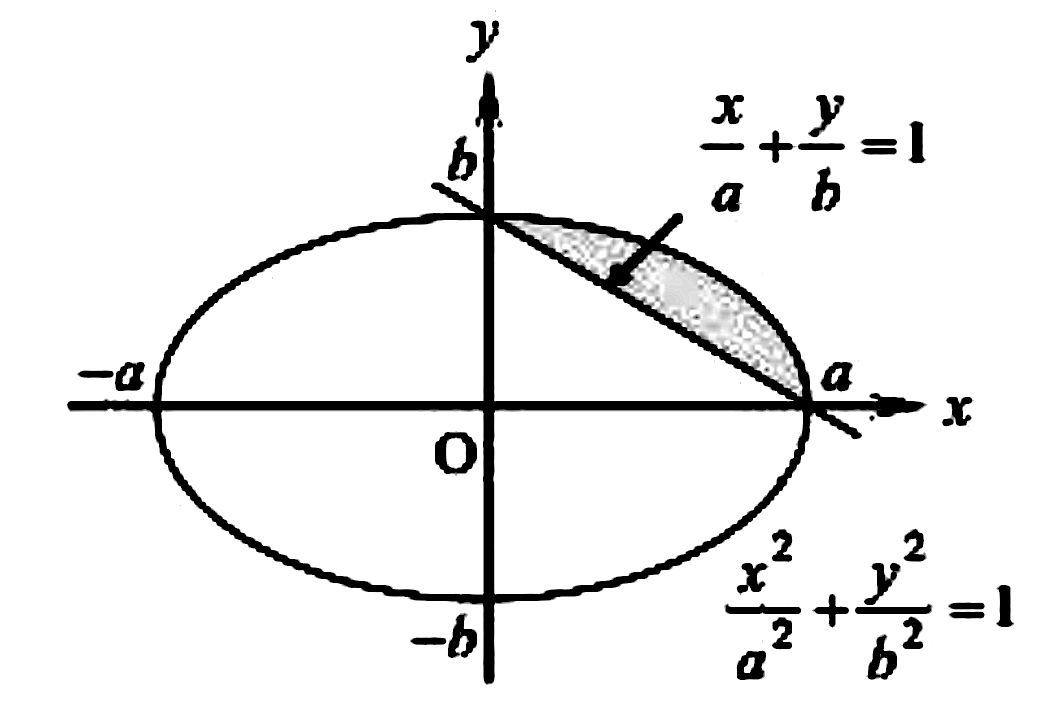
\includegraphics[width=0.35\textwidth]{28-28.4-24.png}
            \end{center}
            \begin{enumerate}
                  \item find $V_x$ and $V_y$. \sol{} \vspace{-0.8cm}
                        \begin{multicols}{2}
                              \begin{flalign*}
                                    V_x & = \pi \int_{0}^{a} \left\{ b^2\left(1 - \frac{x^2}{a^2}\right) - \left[b\left(1 - \dfrac{x}{a}\right)\right]^2\right\} dx & \\
                                        & = b^2 \pi \int_{0}^{a} \left( 1 - \frac{x^2}{a^2} - 1 + \frac{2x}{a} - \frac{x^2}{a^2} \right) dx                         & \\
                                        & = b^2 \pi \int_{0}^{a} \left( \frac{2x}{a} - \frac{2x^2}{a^2} \right) dx                                                  & \\
                                        & = b^2 \pi \left[ \frac{x^2}{a} - \frac{2x^3}{3a^2} \right]_{0}^{a}                                                        & \\
                                        & = b^2 \pi \left( \frac{a^2}{a} - \frac{2a^3}{3a^2} \right) = \frac{\pi ab^2}{3}
                              \end{flalign*}
                              \vfill\null
                              \begin{flalign*}
                                    V_y & = \pi \int_{0}^{b} \left\{ a^2\left(1 - \frac{y^2}{b^2}\right) - \left[a\left(1 - \dfrac{y}{b}\right)\right]^2\right\} dy & \\
                                        & = a^2 \pi \int_{0}^{b} \left( 1 - \frac{y^2}{b^2} - 1 + \frac{2y}{b} - \frac{y^2}{b^2} \right) dy                         & \\
                                        & = a^2 \pi \int_{0}^{b} \left( \frac{2y}{b} - \frac{2y^2}{b^2} \right) dy                                                  & \\
                                        & = a^2 \pi \left[ \frac{y^2}{b} - \frac{2y^3}{3b^2} \right]_{0}^{b}                                                        & \\
                                        & = a^2 \pi \left( \frac{b^2}{b} - \frac{2b^3}{3b^2} \right)  = \frac{\pi a^2b}{3}
                              \end{flalign*}
                              \vfill\null
                        \end{multicols}
                        \vspace{-1cm}

                  \item if $V_x = 2V_y$, find the value of $a:b$. \sol{}
                        \begin{flalign*}
                              \frac{\pi ab^2}{3} & = 2 \cdot \frac{\pi a^2b}{3} & \\
                              b                  & = 2a                         & \\
                              a:b                & = 1:2
                        \end{flalign*}
            \end{enumerate}
\end{enumerate}

\section{Revision Exercise 28}

\begin{enumerate}
    \item $\displaystyle\int_0^a\left(2 x^2-3 x+2\right) d x$
    \item $\displaystyle\int_1^3\left(x^2+\dfrac{1}{x^3}\right) d x$
    \item $\displaystyle\int_{-\dfrac{\pi}{6}}^{\frac{\pi}{2}}(3 \sin \theta-2 \cos 2 \theta) d \theta$
    \item $\displaystyle\int_{-\dfrac{\pi}{4}}^{\frac{\pi}{4}}\left(3 \sec ^2 \theta+\tan ^2 \theta\right) d \theta$
    \item $\displaystyle\int_0^{\ln 2} e^{3 x} d x$
    \item $\displaystyle\int_1^3 \dfrac{2}{3 x-1} d x$
    \item $\displaystyle\int_1^{16} \dfrac{2 x+3}{\sqrt{x}} d x$
    \item $\displaystyle\int_1^4 \dfrac{(\sqrt{x}-1)^2}{x} d x$
    \item $\displaystyle\int_1^2\left(x+\dfrac{4}{x^2}\right)^2 d x$
    \item $\displaystyle\int_0^1 \dfrac{x+1}{x^2+2 x+3} d x$
    \item $\displaystyle\int_{-1}^2 \dfrac{5 x}{\left(1+x^2\right)^4} d x$
    \item $\displaystyle\int_0^2 \dfrac{x}{\sqrt{25-4 x^2}} d x$
    \item $\displaystyle\int_2^4 \dfrac{3 x-2}{(2 x-3)^2} d x$
    \item $\displaystyle\int_2^4 \dfrac{2}{x^3-x} d x$
    \item $\displaystyle\int_1^3 \dfrac{1}{x^3+2 x^2+x} d x$
    \item $\displaystyle\int_0^\pi(\sin \theta+\cos \theta)^2 d \theta$
    \item $\displaystyle\int_0^{\frac{\pi}{3}} \sec ^2 \theta \tan \theta d \theta$
    \item $\displaystyle\int_{-\dfrac{\pi}{2}}^{\frac{\pi}{2}} \sin ^2 \theta \cos \theta d \theta$
    \item $\displaystyle\int_0^1 \dfrac{e^x}{e^x+1} d x$
    \item $\displaystyle\int_{\dfrac{\pi}{6}}^{\frac{\pi}{3}} \dfrac{\sec ^2 \theta}{\tan \theta} d \theta$
    \item Given that $\displaystyle\int_0^4 f(x) d x=2, \displaystyle\int_0^3 g(x) d
              x=4$, and $\displaystyle\int_3^8 g(x) d x=12$. Find the value of
          $\displaystyle\int_0^8\left[f\left(\dfrac{x}{2}\right)-2 g(x)\right] d x$.
    \item Given the function $y=(x+3) \sqrt{2 x-3}$, find $\dfrac{d y}{d x}$. Hence, find
          $\int_2^6 \dfrac{x}{\sqrt{2 x-3}} d x$.
    \item Given the function $y=x \ln x$, find $\dfrac{d y}{d x}$. Hence, find the
          following definite integrals:
          \begin{enumerate}
              \item $\displaystyle\int_1^4 \ln x d x$
              \item $\displaystyle\int_1^4 \ln (2 x) d x$
          \end{enumerate}
    \item Find the area of the region bounded by the curve $y=\dfrac{1}{x+1}$, the lines
          $x=1, x=7$, and the $x$-axis.
    \item Find the area of the region bounded by the curve $y=\dfrac{3}{x}$ and the line
          $y=4-x$.
    \item Find the area of the region bounded by the curve $x=y^2-5 y$ and the line $x+7
              y=24$.
    \item Find the area of the region bounded by the curves $y=x^2$ 及 $y^3=x$.
    \item Shown in the diagram below is the shaded region bounded by the curves $y=\ln x,
              y=\ln (2 x-1)$, and the line $y=3$. Find the area of this region.
    \item Find the area of the region bounded by the curves $x=y^3-y$ 及 $x=y-y^2$.
    \item Shown in the diagram below is the shaded region bounded by the curves $y=\sin
              x$ 及 $y=\sin 2 x$ in the interval $0 \leq x \leq \pi$. Find the area of this
          region.
    \item Find the volume of the solid of revolution formed by rotating the region
          bounded by the curve $y=\frac{1}{x+2}$, the line $x=2$, and two axes about the
          $x$-axis.
    \item Find the volume of the solid of revolution formed by rotating the region
          bounded by the curve $y=e^x-3$ and the two axes about the $x$-axis.
    \item Find the volume of the solid of revolution formed by rotating the region
          bounded by the curve $x=y^2-3 y$ and the $y$-axis about the $y$-axis.
    \item Find the volume of the solid of revolution formed by rotating the region
          bounded by the curve $y=x^2$ and the line $y=x+2$ about the $x$-axis.
    \item Find the volume of the solid of revolution formed by rotating the region
          bounded by the curve $y^2=x+9$ and the line $y=x+3$ about the $y$-axis.
    \item Given that a region is bounded by the curve $y^2=8 x$ and $y=x^2$. Find the
          volume of the solid of revolution formed by rotating this region about the
          $x$-axis and the $y$-axis respectively.
    \item SHown in the diagram below is the shaded region bounded by the curve $y =
              2\cos\pi x$, the line $y = 3x$, and the $y$-axis.
          \begin{enumerate}
              \item Prove that the $x$-coordinate of point $A$ is $\dfrac{1}{3}$.
              \item Find the volume of the solid of revolution formed by rotating this region about
                    the $x$-axis.
          \end{enumerate}
    \item Given that a region is bounded by the curve $xy = 12$, the line $x = 4$, and $y
              = 6$. Find the volume of the solid of revolution formed by rotating this region
          about the $x$-axis and the $y$-axis respectively.
\end{enumerate}